\section{Systematic Uncertainties}
\def\effTri{\ensuremath{\epsilon_{\mathrm{trigger}}}\xspace}
\def\effTotJ{\ensuremath{\epsilon_{\mathrm{tot,\jpsi}}}\xspace}
\def\effTotP{\ensuremath{\epsilon_{\mathrm{tot,\psitwos}}}\xspace}
\def\pandb{prompt components and components from $b$-hadron decay}
The ratio of production of \psitwos to \jpsi in a certain $(\pt,y)$ is 
defined in equation ~\ref{Rsingle}, which is universal for both prompt components and components from $b$-hadron decay in each multiplicity bin and
Systematic uncertainties of various sources are combined through the error propagation formula in each bin.
While when calculating the systematic uncertainties of the ratio of integrated production, the bin size is 
no more canceled and we need to take into account the production as weight in each bin. The ratio of integrated 
production is defined in equation ~\ref{Rintegrated}.

The form of expression for the ratio of integrated production is not a simple production or division (it is a division of sums). So when studying the systematic uncertainties, 
a simple and straightforward way is calculating the uncertainties of $\frac{\Sigma_{(\pt,y)}\sigma_{\psitwos}(\pt,y)}{\Sigma_{(\pt,y)}\sigma_{\jpsi}(\pt,y)}$ itself, 
which is for example, if we calculate the uncertainty of the fit model, instead of combining the uncertainties from 
different bins, we directly calculate how much $\frac{\Sigma_{(\pt,y)}\sigma_{\psitwos}(\pt,y)}{\Sigma_{(\pt,y)}\sigma_{\jpsi}(\pt,y)}$ 
would vary when we change the fit model. For the uncertainties which are independent of bins, we can 
combine them through the error propagation formula, i.e. the Systematic uncertainty due to MC sample size.
The following sources of systematic uncertainties are considered. And the systematic uncertainties are calculated 
separately in each multiplicity bin.
For the rest of the part, we only show the results for the first multiplicity bin, which is 4$\leq$PVNTRACKS$<$20. 
%=============================================================================================
\subsection{Signal extraction}
\subsubsection{Signal mass shape}
\label{sec:masssyst}
Using the sum of two Crystal Ball functions parametrized as described in Section~\ref{Signal Extraction} could bias the signal yields.
For an alternative, the signal invariant mass is also fitted with the model which is extracted from the kernel-estimated distribution from the simulated sample bin dependently. 
In order to account for the resolution difference between data and simulation, a Gaussian function (all the parameters float during the fit procedure) is used to smear the shape of the signals.
The study is performed in each kinematic bin, and the signal yields from the default fit and alternative fit are compared.
For both \jpsi and \psitwos, we change the fit model to get uncertainties for both and then calculate the uncertainties through the error propagation formula.
The detailed results of systematic uncertainty for ratio in each single $\pt$ and $y$ bin and PVNTRACKS from 4 to 20 are shown in Fig.~\ref{sys_mass}.
The result is common for both prompt components and components from $b$-hadron decay since when we fit the mass spectrum, we fit both components simultaneously. 
\begin{figure}[!tbp]
    \begin{center}
      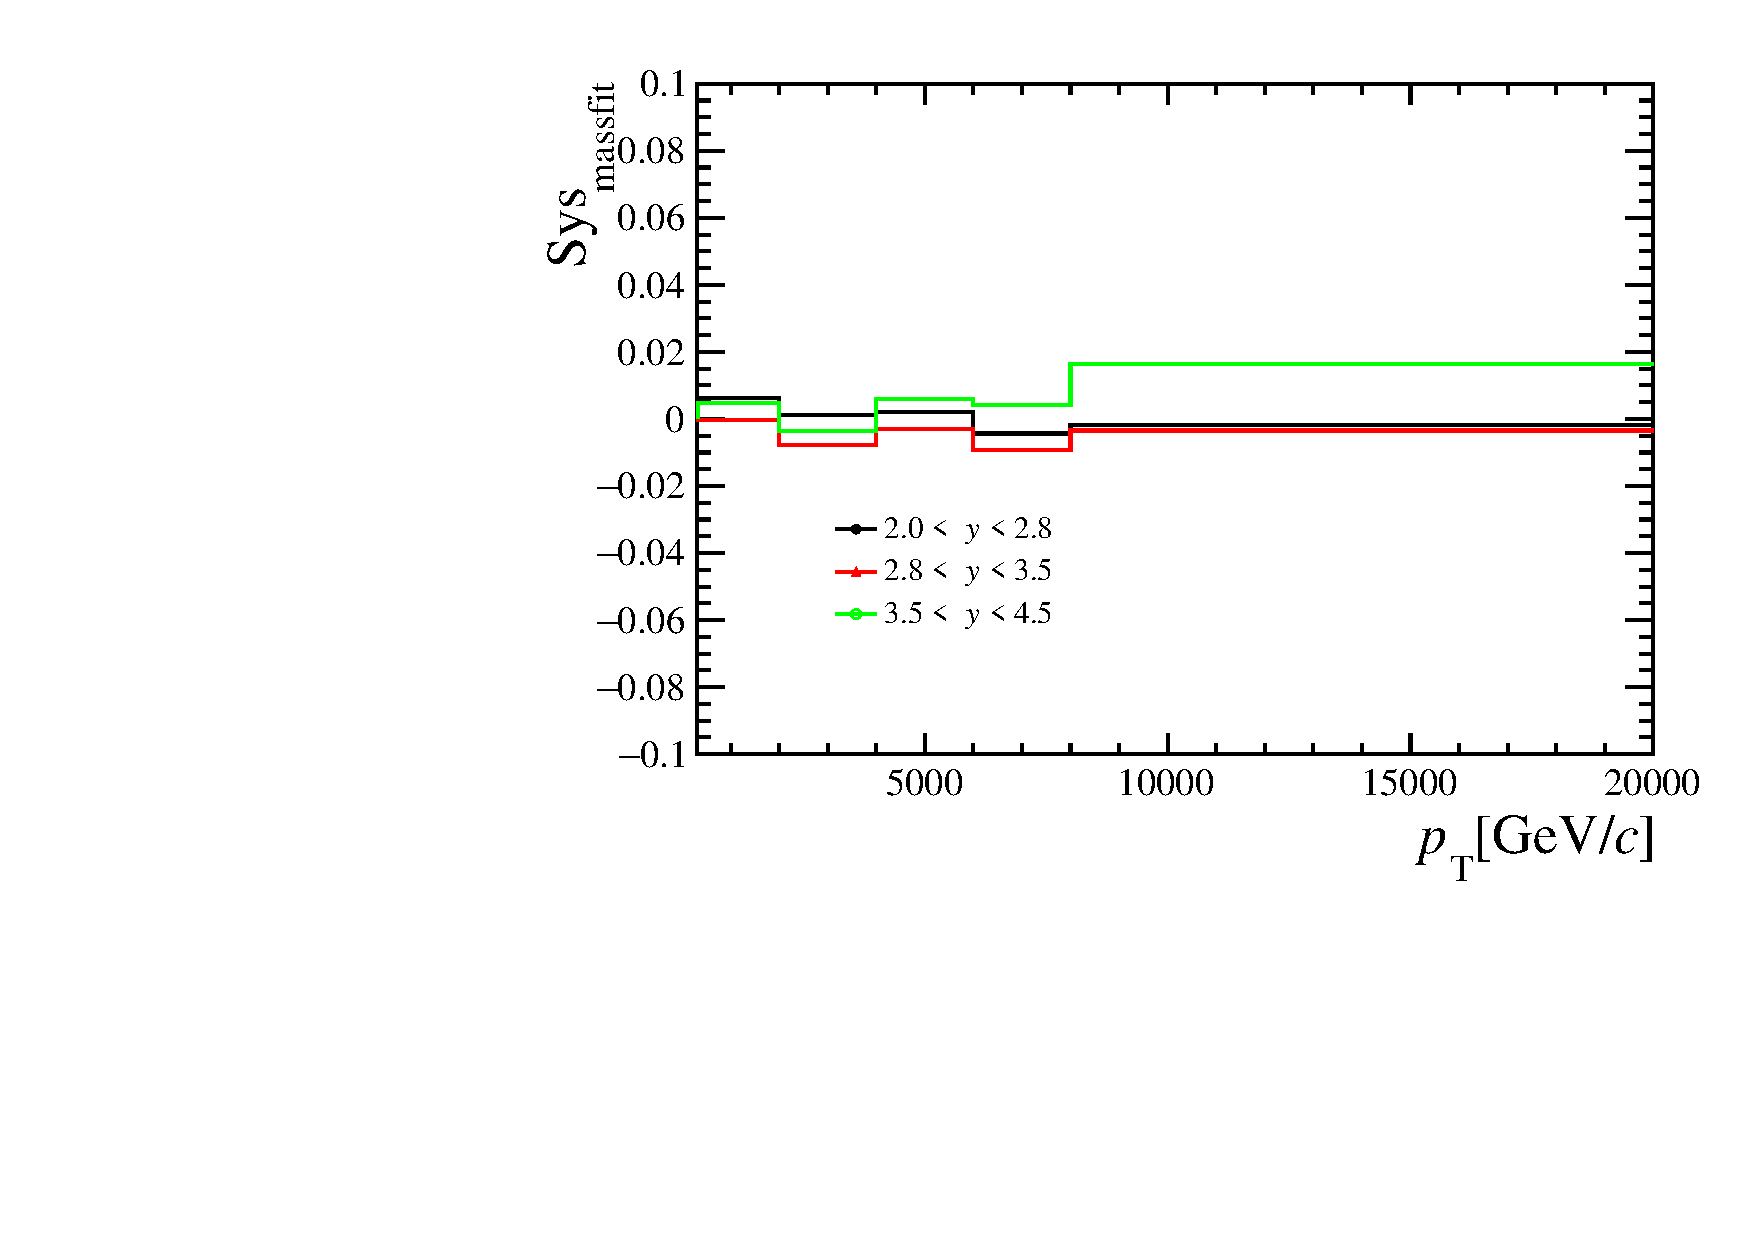
\includegraphics[width=0.49\linewidth]{pdf/SysMPlot/n1Err_point.pdf}
      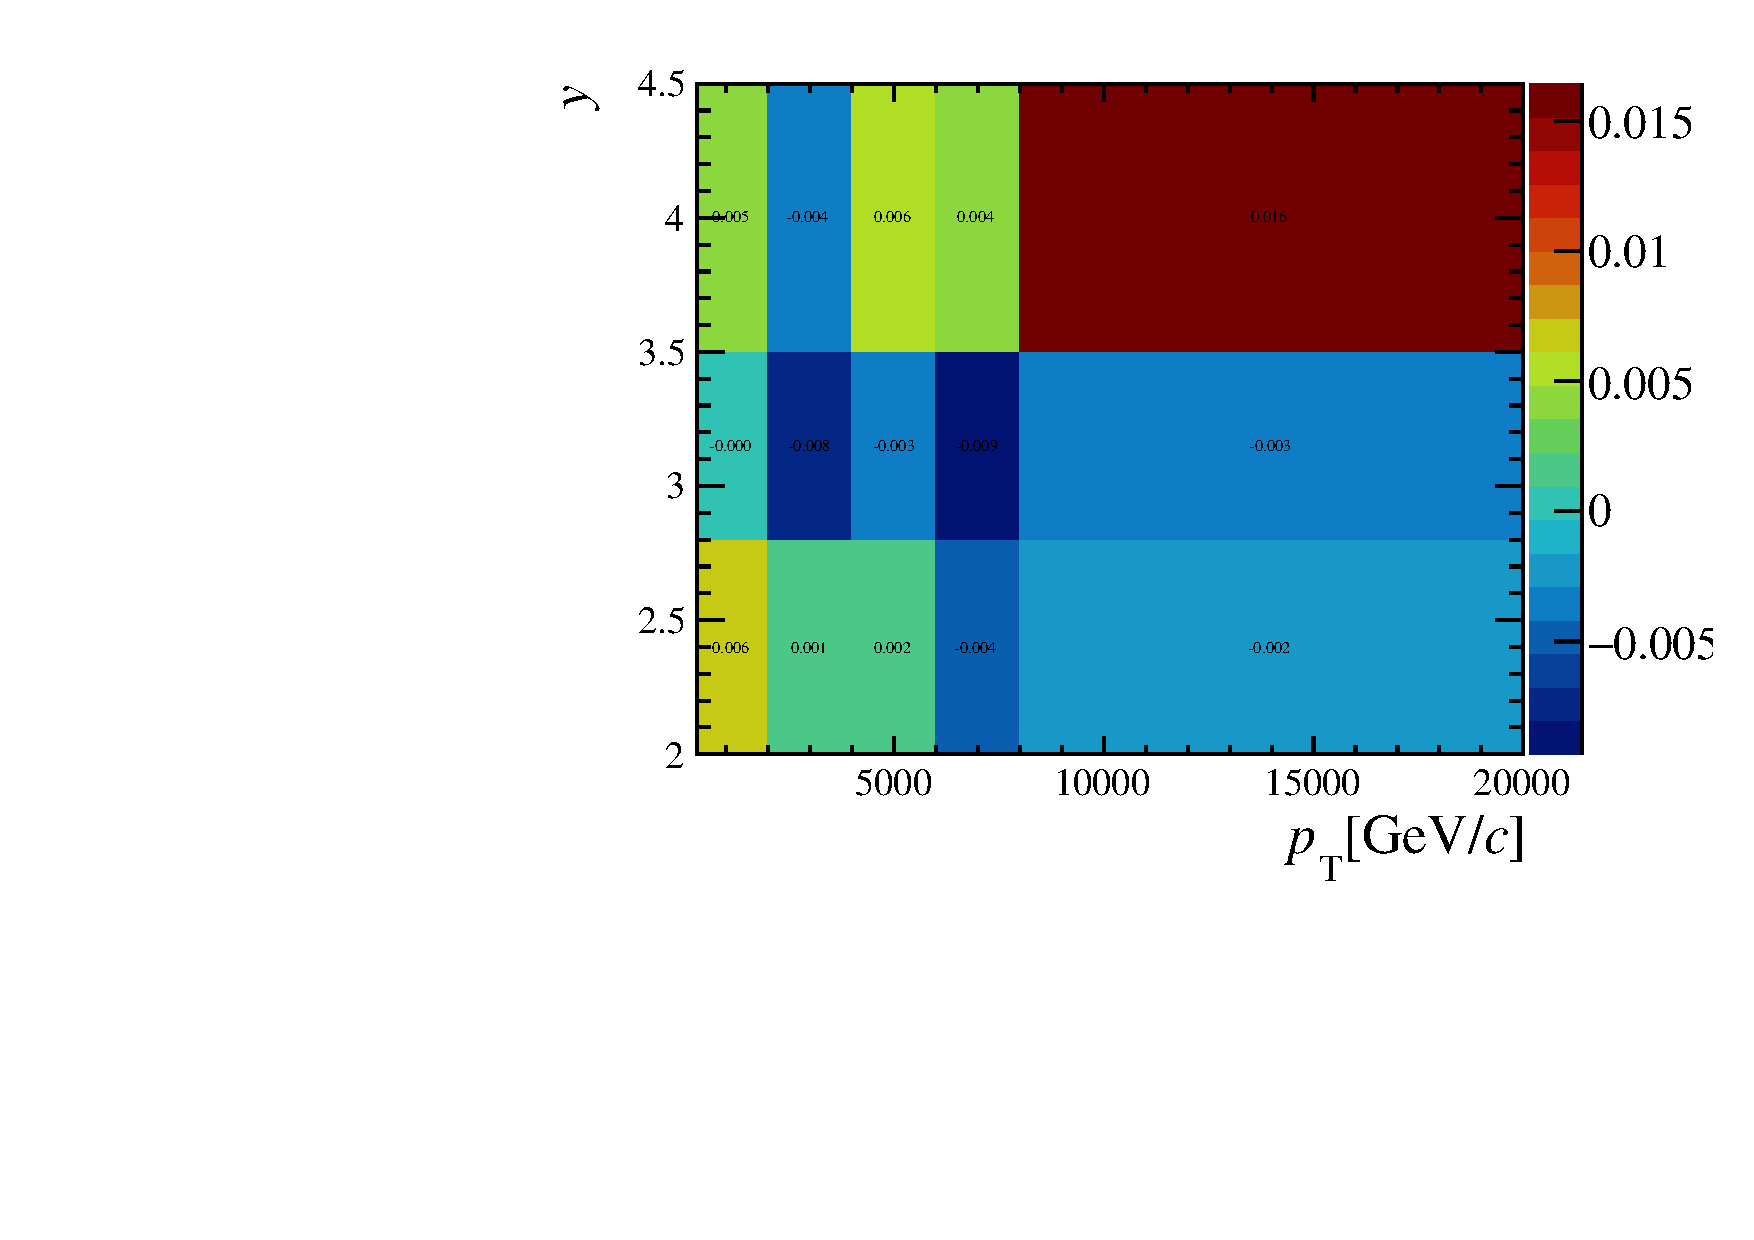
\includegraphics[width=0.49\linewidth]{pdf/SysMPlot/n1Err.pdf}
    \end{center}
    \caption{The systematic uncertainty of ratio of production due to the fit model in each bin for PVNTRACKS from 4 to 20. It is common for both prompt components and components from $b$-hadron decay.
      }
    \label{sys_mass}
\end{figure}
For the ratio of integrated production, we change the fit model and calculate a new value with equation~\ref{Rintegrated}. The variation 
between the new ratio and the original one is quoted as systematic uncertainty for ratio of integrated production due to mass fit model. 


\subsubsection{Fit to $t_z$ background}
\label{sec:tzsyst}
There are several scenarios that could deviate the fitted $\bquark$ fraction from its true value:  
\begin{itemize}

\item Imperfect modeling of the detector resolution of $t_z$. 
Since the shape of prompt \psitwos is dominated by the resolution, a defective description of the resolution could make the prompt 
\jpsi and \psitwos distribution not fitted very well, and thus will affect the fitted fraction of components from $\bquark$. 
To study this effect, a third wide Gaussian is added to the resolution function.
It is found that the difference of the fitted $F_b$ between the default fit and the new fit is negligible.

\item Systematic uncertainty related to the background description. 
In the nominal procedure, the fit explicitly models the background distribution using the mass sidebands. 
As an alternative, the parameters of the $t_z$ distribution for the background are obtained by the sPlot technique for both \jpsi and \psitwos and are fixed in the $t_z$ fit.
\end{itemize}

For each $\pt$ and $y$ bin, the systematic uncertainties are calculated by combining the uncertainties from \jpsi and \psitwos. For 
the ratio of integrated production, similarly, as above, we change the fit model for $t_z$ background for both \jpsi and \psitwos to calculate a 
new value and quote the variation as a systematic uncertainty. The uncertainties for \pandb are calculated separately.
The results in a single bin are shown in figure~\ref{sys_tzbkg}. 
\begin{figure}[!tbp]
    \begin{center}
      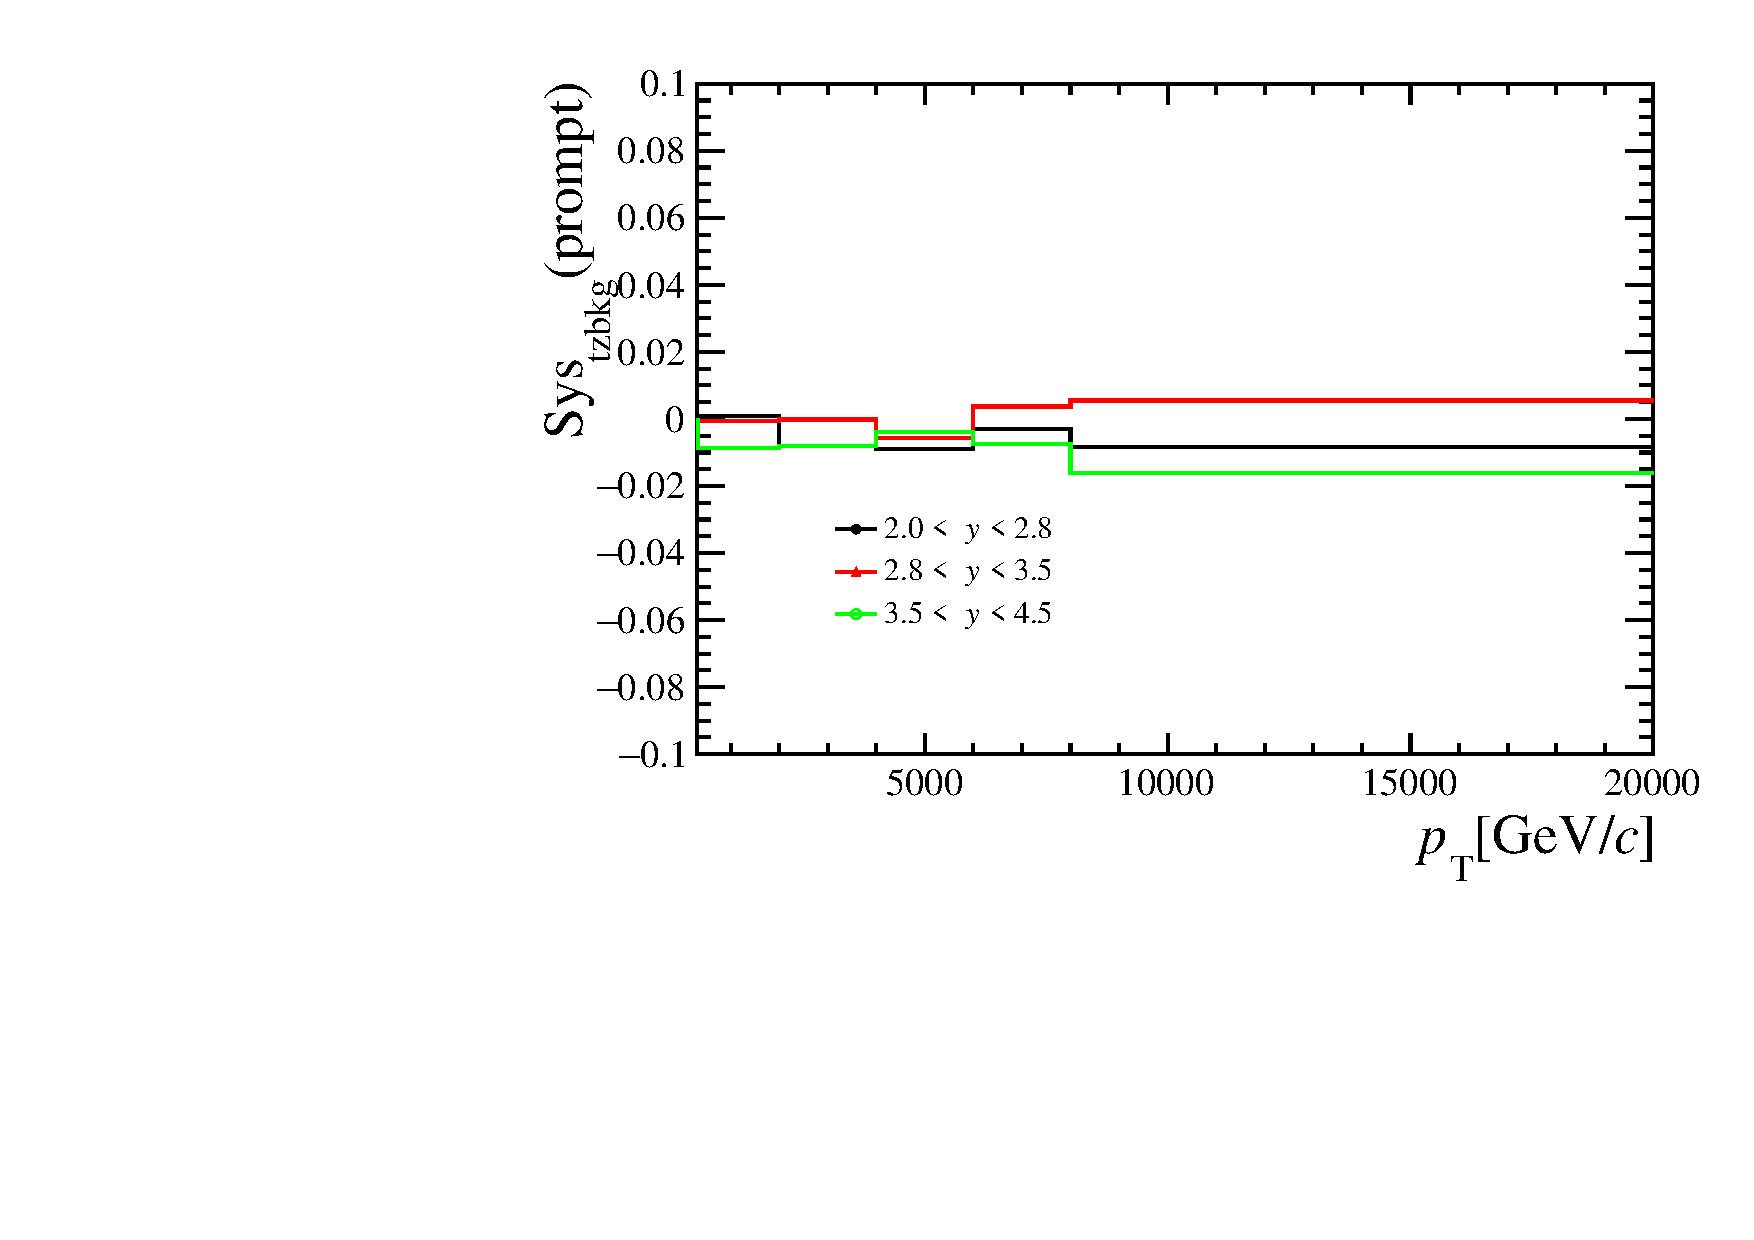
\includegraphics[width=0.49\linewidth]{pdf/SysTzPlot/tzbkg/n1Errp_point.pdf}
      \includegraphics[width=0.49\linewidth]{pdf/SysTzPlot/tzbkg/n1Errp.pdf}
      \vspace*{-0.5cm}
      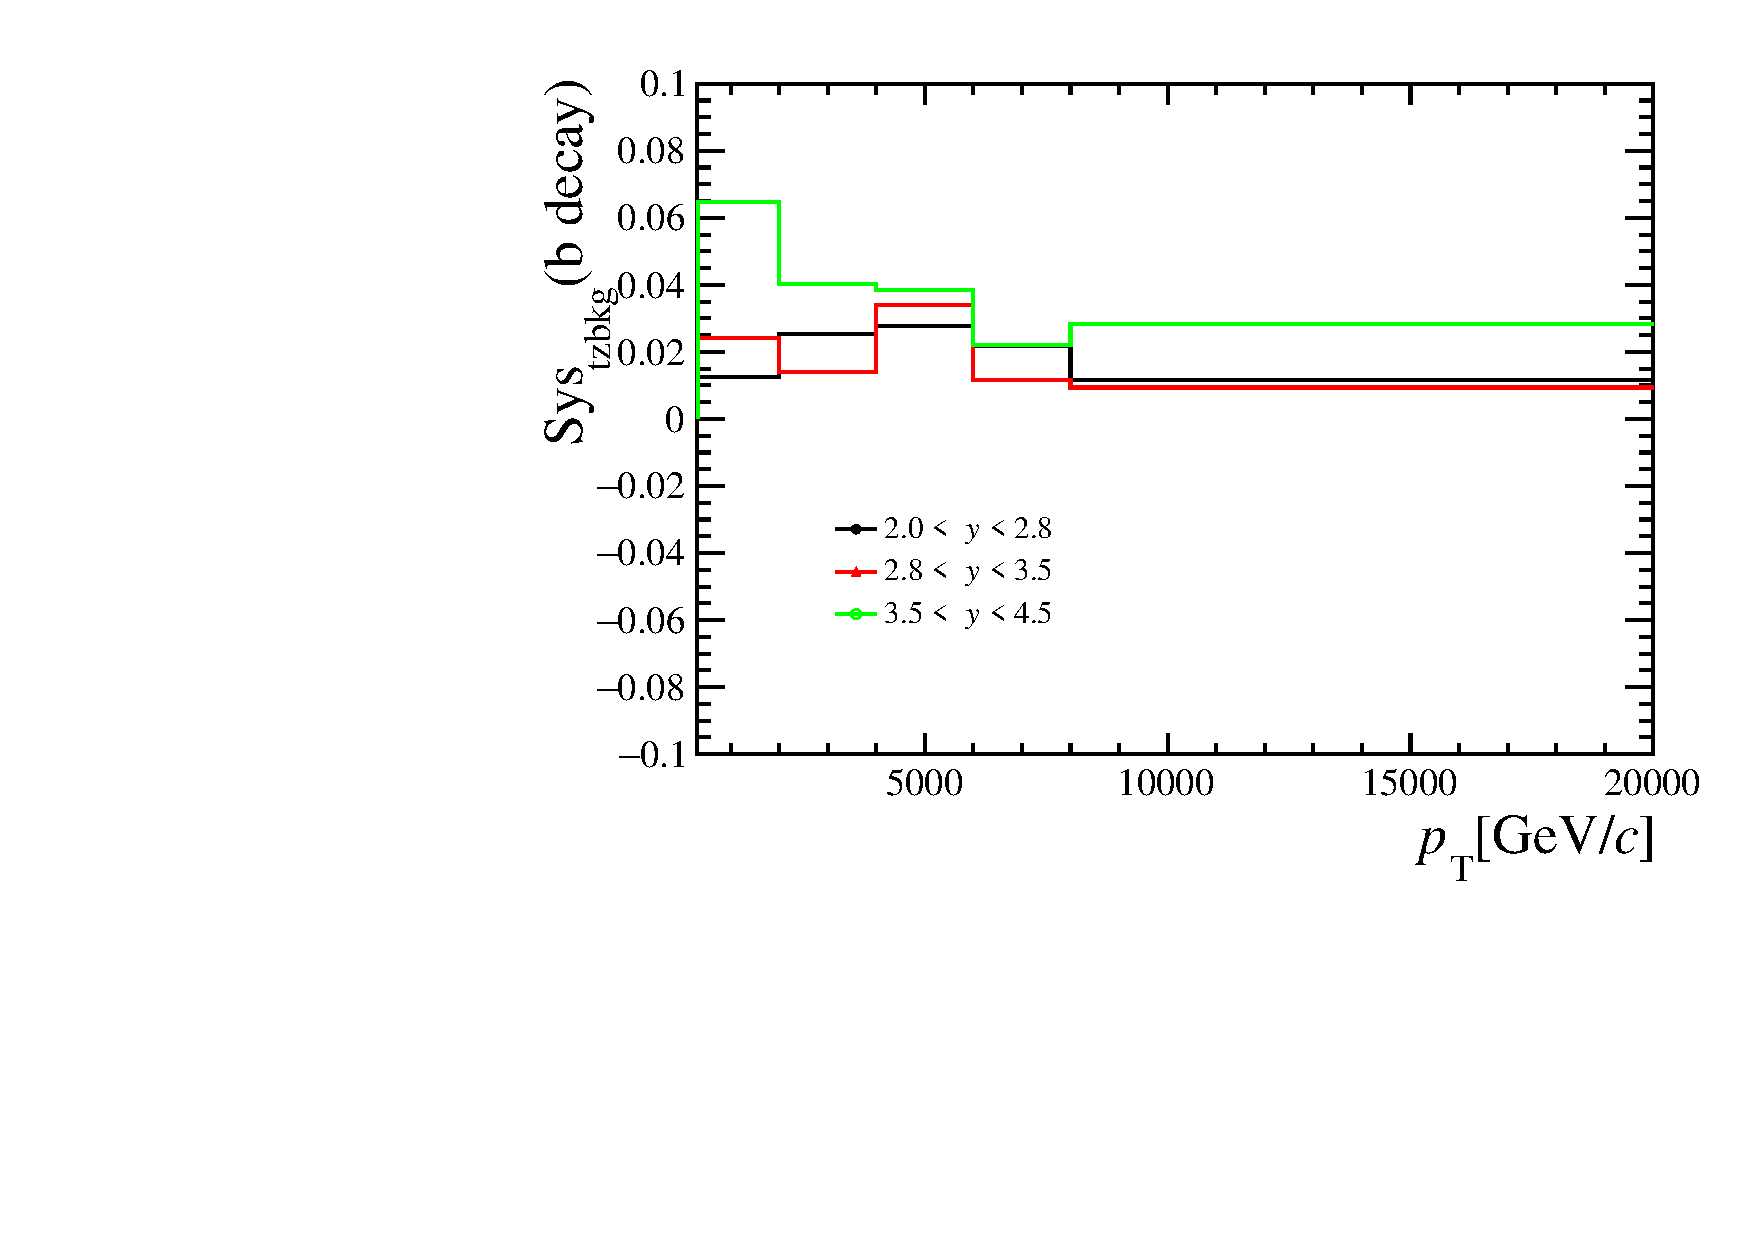
\includegraphics[width=0.49\linewidth]{pdf/SysTzPlot/tzbkg/n1Errb_point.pdf}
      \includegraphics[width=0.49\linewidth]{pdf/SysTzPlot/tzbkg/n1Errb.pdf}
    \end{center}
    \caption{The systematic uncertainty of ratio of production due to $t_z$ background fit model in each bin for PVNTRACKS from 4 to 20. The first row is that of prompt components and the second row is that of components from $b$-hadron decay.
      }
    \label{sys_tzbkg}
\end{figure}

% \begin{table}[h]
%     \centering
%     \caption{Summary of systematic uncertainties of ratio of integrated production due to the model of $t_z$ background for PVNTRACKS from 4 to 20.}
% \begin{center}
%     \begin{tabular}{ c | c | c }
%         \hline
%         Region & prompt (\%) & from $b$ (\%)\\
%         \hline
%         2.0$<$y$<$2.8&1.08&-0.38\\
%         2.8$<$y$<$3.5&-0.26&2.46\\
%         3.5$<$y$<$4.5&1.31&-0.26\\
%         \hline
%         0\gevc $<$\pt$<$2\gevc&0.55&0.59\\
%         2\gevc $<$\pt$<$4\gevc&1.18&-0.39\\
%         4\gevc $<$\pt$<$6\gevc&0.60&1.34\\
%         6\gevc $<$\pt$<$8\gevc&-0.41&1.73\\
%         8\gevc $<$\pt$<$20\gevc&-0.68&1.52\\
%         \hline
%         all \pt-y region&0.76&0.50\\
%         \hline
%     \end{tabular}
% \end{center}
% \label{sys_tzbkg_int}
% \end{table}

\subsubsection{Fit to $t_z$ signal}
\label{sec:tzsig}
For the imperfect modeling of detector resolution, we fit the $t_z$ spectrum on MC and then 
compare the yields of prompt components to the real counts in MC. The variation is quoted as 
systematic uncertainty due to imperfect modeling of the $t_z$ signal model. When fitting the $t_z$ spectrum on MC for \jpsi or \psitwos, we should take care that one or two Gaussian functions 
should be used depending on the number of Gaussian functions we are using when fitting $t_z$ spectrum on data in a certain (\pt,$y$, PVNTRACKS) bin.
The systematic uncertainties of ratio in different bins~\ref{sys_tzsig} are 
listed for PVNTRACKS from 4 to 20.
\begin{figure}[!tbp]
    \begin{center}
      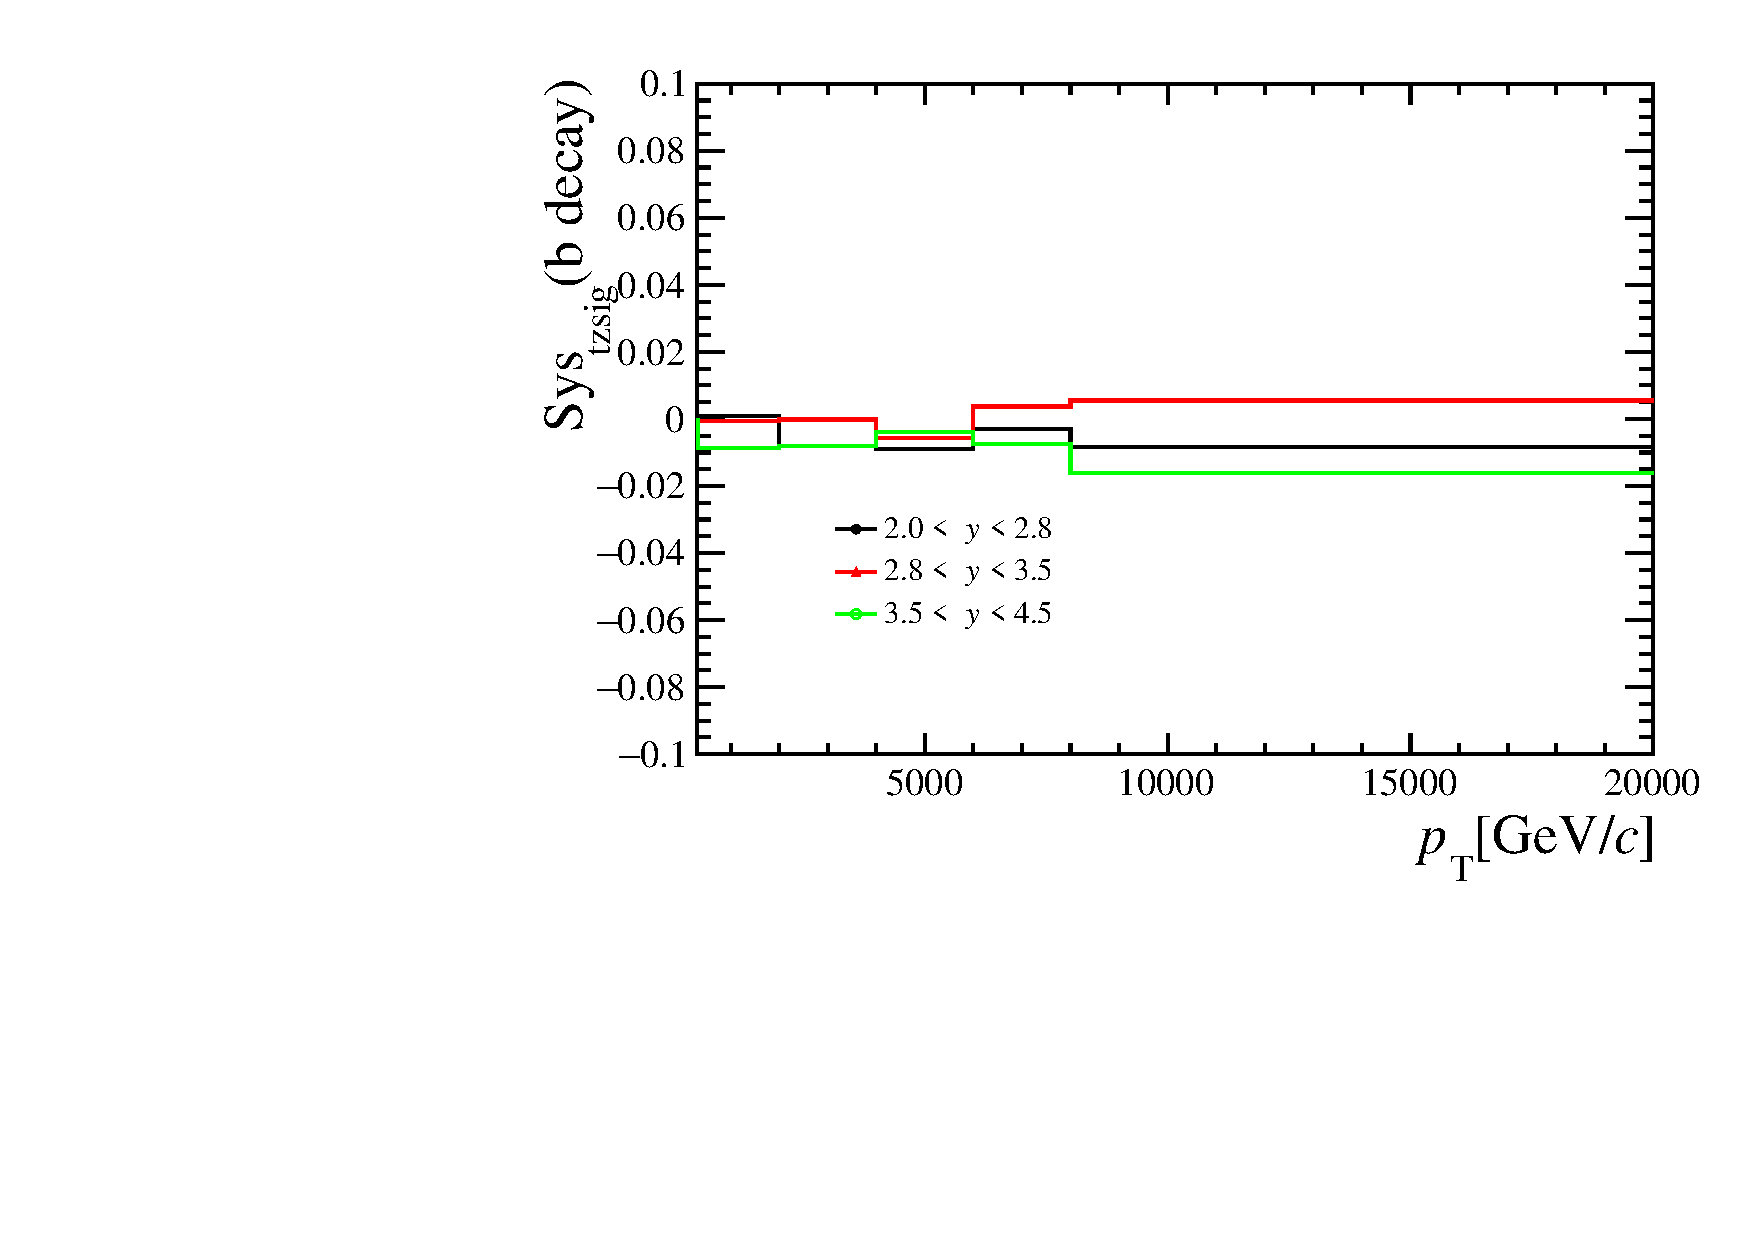
\includegraphics[width=0.49\linewidth]{pdf/SysTzPlot/tzsig/n1Errp_point.pdf}
      \includegraphics[width=0.49\linewidth]{pdf/SysTzPlot/tzsig/n1Errp.pdf}
      \vspace*{-0.5cm}
      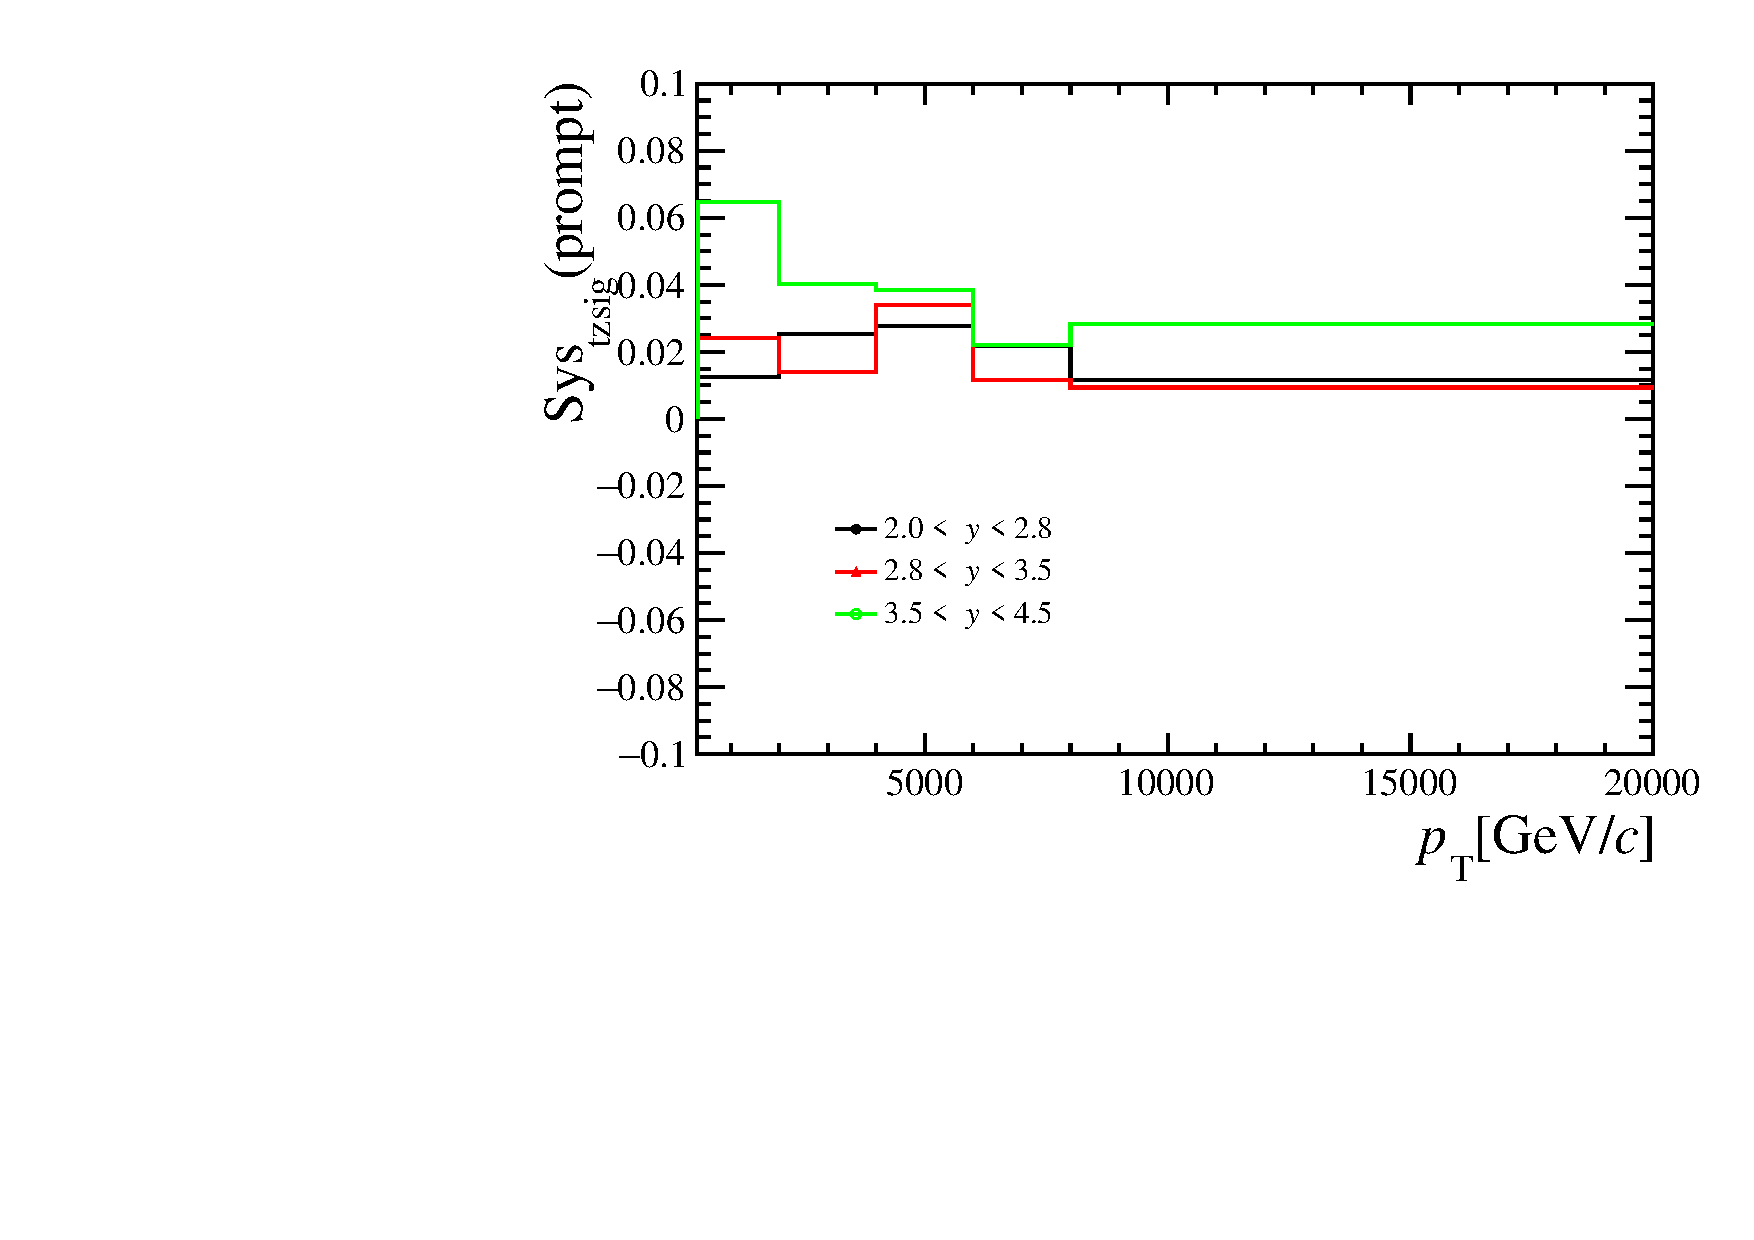
\includegraphics[width=0.49\linewidth]{pdf/SysTzPlot/tzsig/n1Errb_point.pdf}
      \includegraphics[width=0.49\linewidth]{pdf/SysTzPlot/tzsig/n1Errb.pdf}
    \end{center}
    \caption{The systematic uncertainty of ratio of production due to $t_z$ signal fit model in each bin for PVNTRACKS from 4 to 20. The first row is that of prompt components and the second row is that of components from $b$-hadron decay.
      }
    \label{sys_tzsig}
\end{figure}

% \begin{table}[h]
%     \centering
%     \caption{Summary of systematic uncertainties of ratio of integrated production due to the model of $t_z$ signal for PVNTRACKS from 4 to 20.}
% \begin{center}
%     \begin{tabular}{ c | c | c }
%         \hline
%         Region & prompt (\%) & from $b$ (\%)\\
%         \hline
%         2.0$<$y$<$2.8&1.91&0.20\\
%         2.8$<$y$<$3.5&1.04&-0.08\\
%         3.5$<$y$<$4.5&0.58&-0.32\\
%         \hline
%         0\gevc $<$\pt$<$2\gevc&1.41&-0.01\\
%         2\gevc $<$\pt$<$4\gevc&1.18&-0.82\\
%         4\gevc $<$\pt$<$6\gevc&-0.60&0.55\\
%         6\gevc $<$\pt$<$8\gevc&1.95&-2.76\\
%         8\gevc $<$\pt$<$20\gevc&1.23&-0.66\\
%         \hline
%         all \pt-y region&1.22&0.04\\
%         \hline
%     \end{tabular}
% \end{center}
% \label{sys_tzsig_int}
% \end{table}

%=============================================================================================

\subsection{Trigger efficiency}
The trigger efficiency in simulation is cross-checked with data, and the resulting difference in the ratio of production between simulation and data is quoted as a systematic uncertainty. 
For both \texttt{L0DiMuon} and \texttt{Hlt1DiMuonHighMass} the TISTOS method is used to evaluate the efficiency for \texttt{L0DiMuon}\&\&\texttt{Hlt1DiMuonHighMass} both in simulation and data. 
We use \texttt{L0Global} and \texttt{Hlt1Global} as the TIS line.
As the data sample size is limited by the number of the TIS events of \psitwos sample, we only consider the uncertainty in different multiplicity bins. 
By comparing the difference between the calculated efficiencies using TISTOS method in data and MC, we construct an estimate of the difference in trigger efficiency calculate by MC and the true trigger efficiency. It is shown in Figs.~\ref{Sys_Trigger_N}.
\begin{figure}[H]
  \begin{center}
  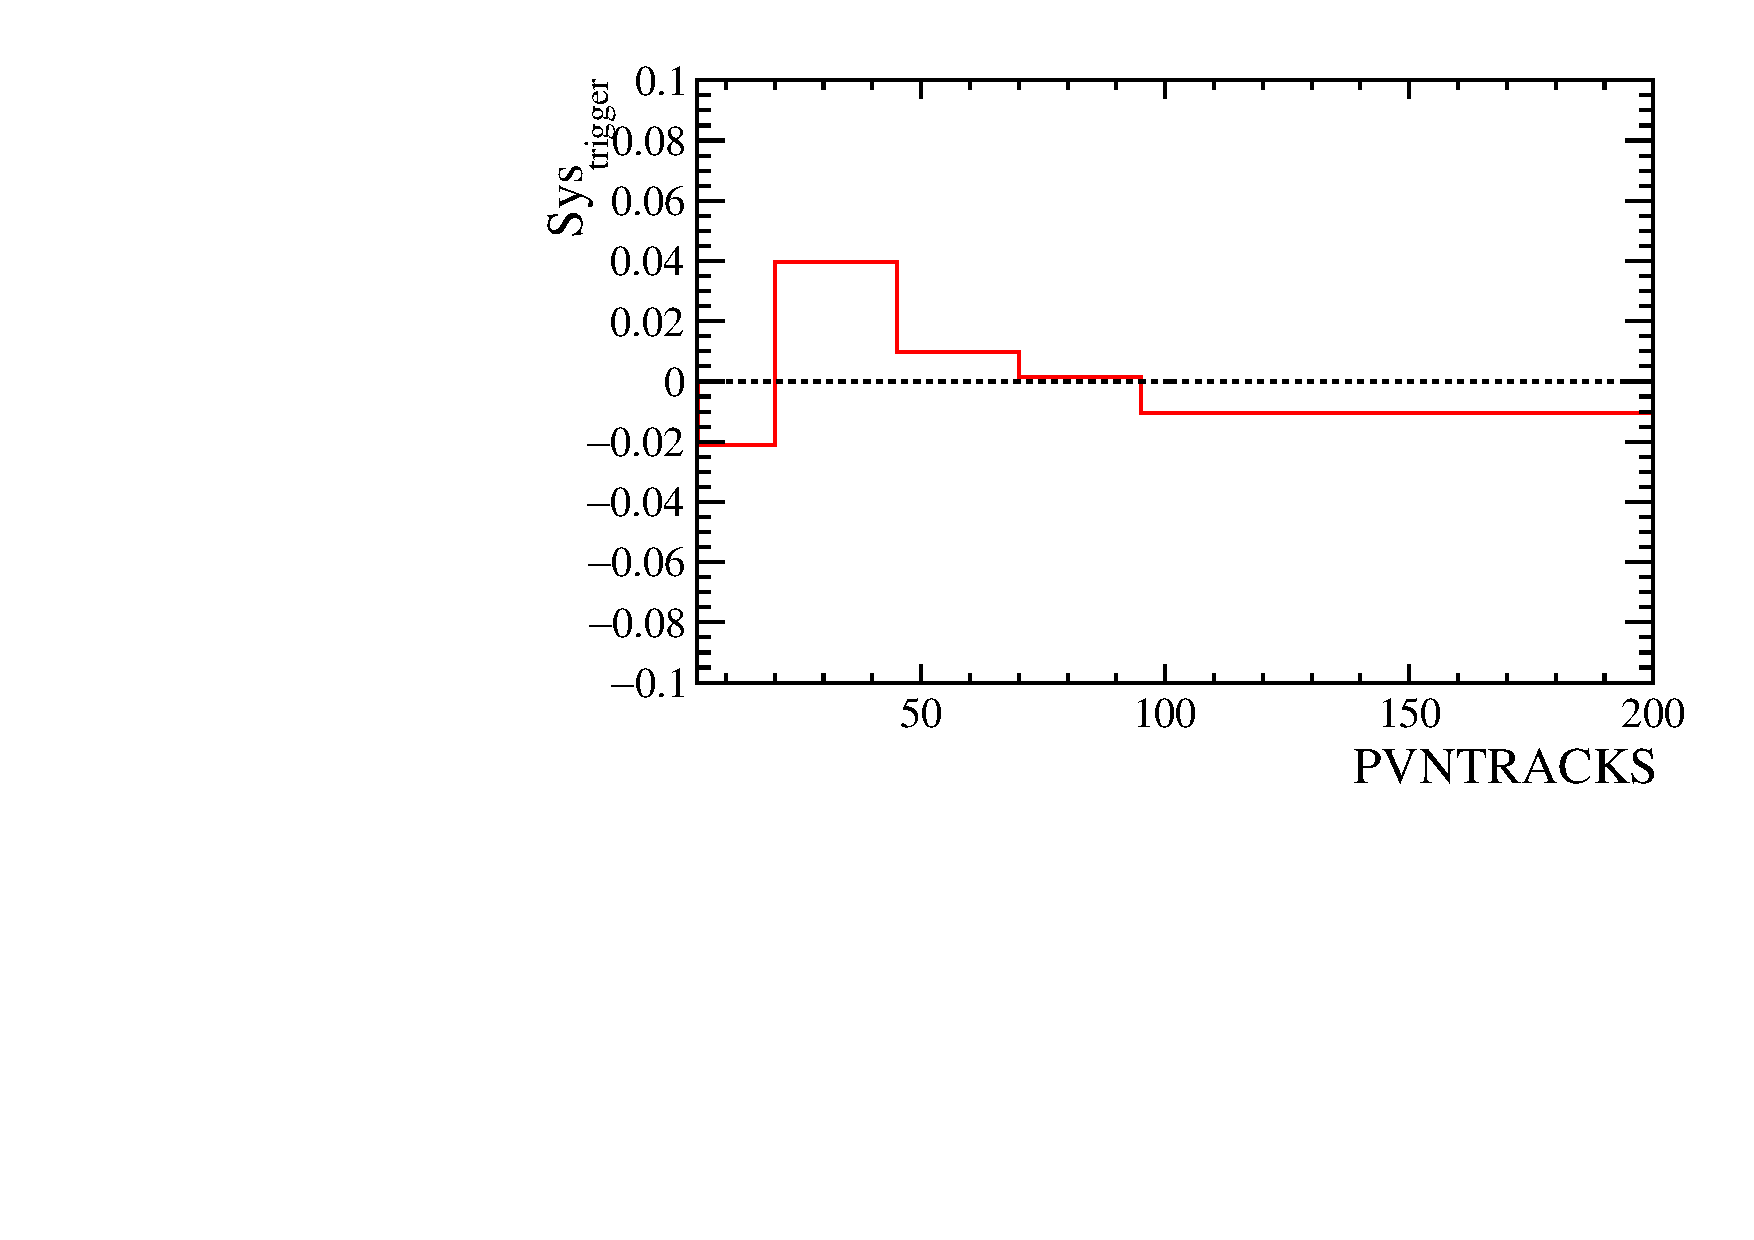
\includegraphics[width=0.8\linewidth, totalheight=0.35\textheight]{pdf/SysTri_PVN.pdf}
  \end{center}
  \caption{
    Summary of Systematic Uncertainties of ratio due to uncertainty of \effTri in differet multiplicity region.}
  \label{Sys_Trigger_N}
\end{figure}
To compare the ratio as a function of \pt with other measurements in different collision systems, we also find the systematic uncertainties in different \pt bins, where we integrate over the multiplicity and rapidity dimensions due to the limit of TIS sample size. It is shown in Figs.~\ref{Sys_Trigger}.
\begin{figure}[H]
  \begin{center}
    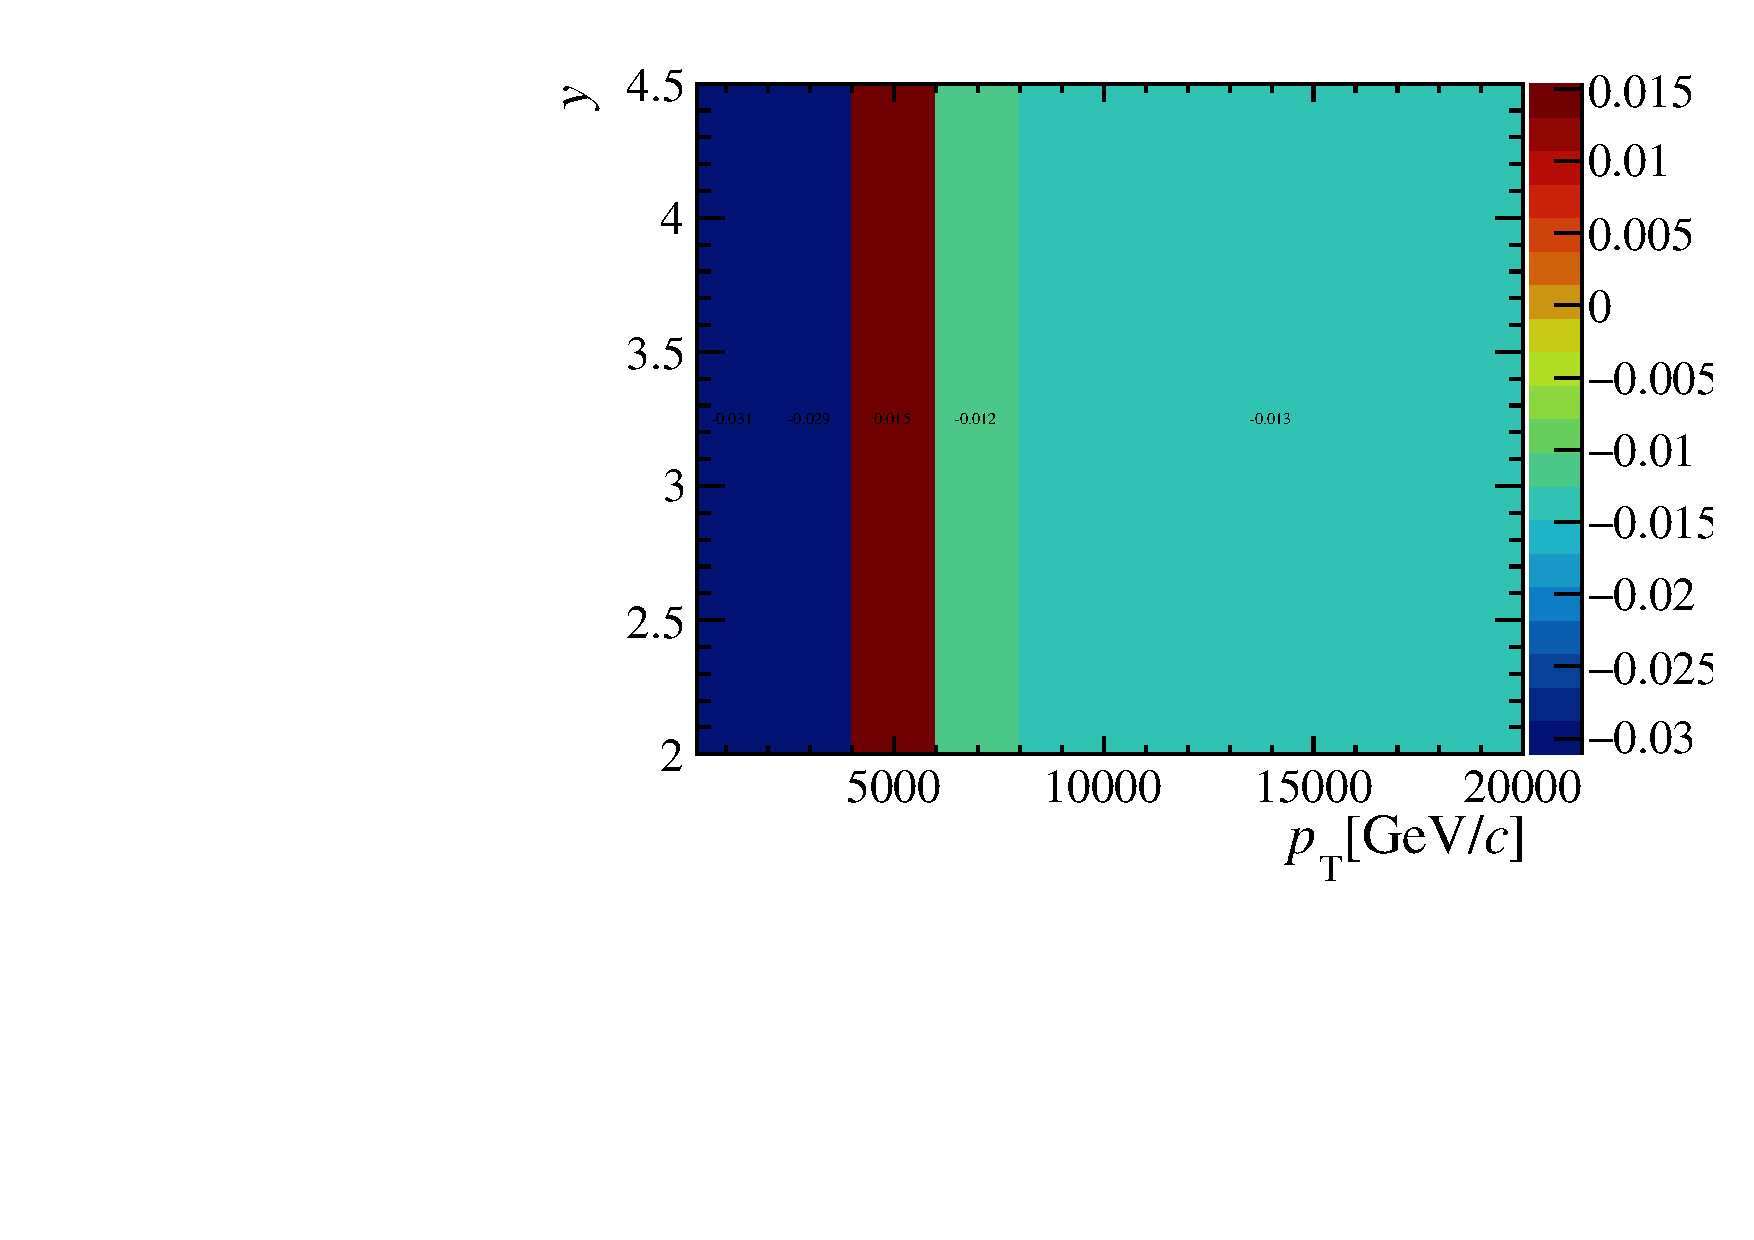
\includegraphics[width=0.8\linewidth,totalheight=0.35\textheight]{pdf/TISTOS.pdf}
  \end{center}
  \caption{
    Summary of Systematic Uncertainties of ratio due to uncertainty of \effTri.}
  \label{Sys_Trigger}
\end{figure}

% \begin{table}[h]
%     \centering
%     \caption{Summary of systematic uncertainties of ratio of integrated production determined by TISTOS method for PVNTRACKS from 4 to 20.}
% \begin{center}
%     \begin{tabular}{ c | c | c }
%         \hline
%         Region & prompt (\%) & from $b$ (\%)\\
%         \hline
%         2.0$<$y$<$2.8&2.82&2.73\\
%         2.8$<$y$<$3.5&2.80&2.81\\
%         3.5$<$y$<$4.5&2.80&2.84\\
%         \hline
%         0\gevc $<$\pt$<$2\gevc&2.70&2.70\\
%         2\gevc $<$\pt$<$4\gevc&2.70&2.70\\
%         4\gevc $<$\pt$<$6\gevc&3.58&3.58\\
%         6\gevc $<$\pt$<$8\gevc&1.02&1.02\\
%         8\gevc $<$\pt$<$20\gevc&0.24&0.24\\
%         \hline
%         all \pt-y region&2.81&2.79\\
%         \hline
%     \end{tabular}
% \end{center}
% \label{Sys_Trigger_int}
% \end{table}

\subsection{Tracking efficiency}
\label{sec:SysTracking}
There are two sources of systematic uncertainties associated with the track reconstruction efficiency. 

One is the statistical uncertainty of the ratios due to the limited sample size used to obtain the tracking correction table.
This part could be obtained by toy studies: 
Two hundred experiments were performed where the efficiency for each bin in the $p$ and $\eta$ was sampled from Fig.~\ref{TrackEfficiencyCalib} by Gaussian distributions with the corresponding central value as the mean and the uncertainty as the width; 
For each experiment, the reconstruction and selection efficiency of\pandb in different bins could be obtained with the sampled efficiency correction table, and hence we can calculate two hundred values for ratio in a single bin or any integrated region; 
Finally, using a gaussian function to fit the two hundred of results, and the sigma divided by the mean value of the fit result is quoted as the relative uncertainty. 
The relative uncertainty in each bin for \pandb for PVNTRACKS from 4 to 20 is shown in figure~\ref{Sys_Tracking1}.
\begin{figure}[!tbp]
    \begin{center}
      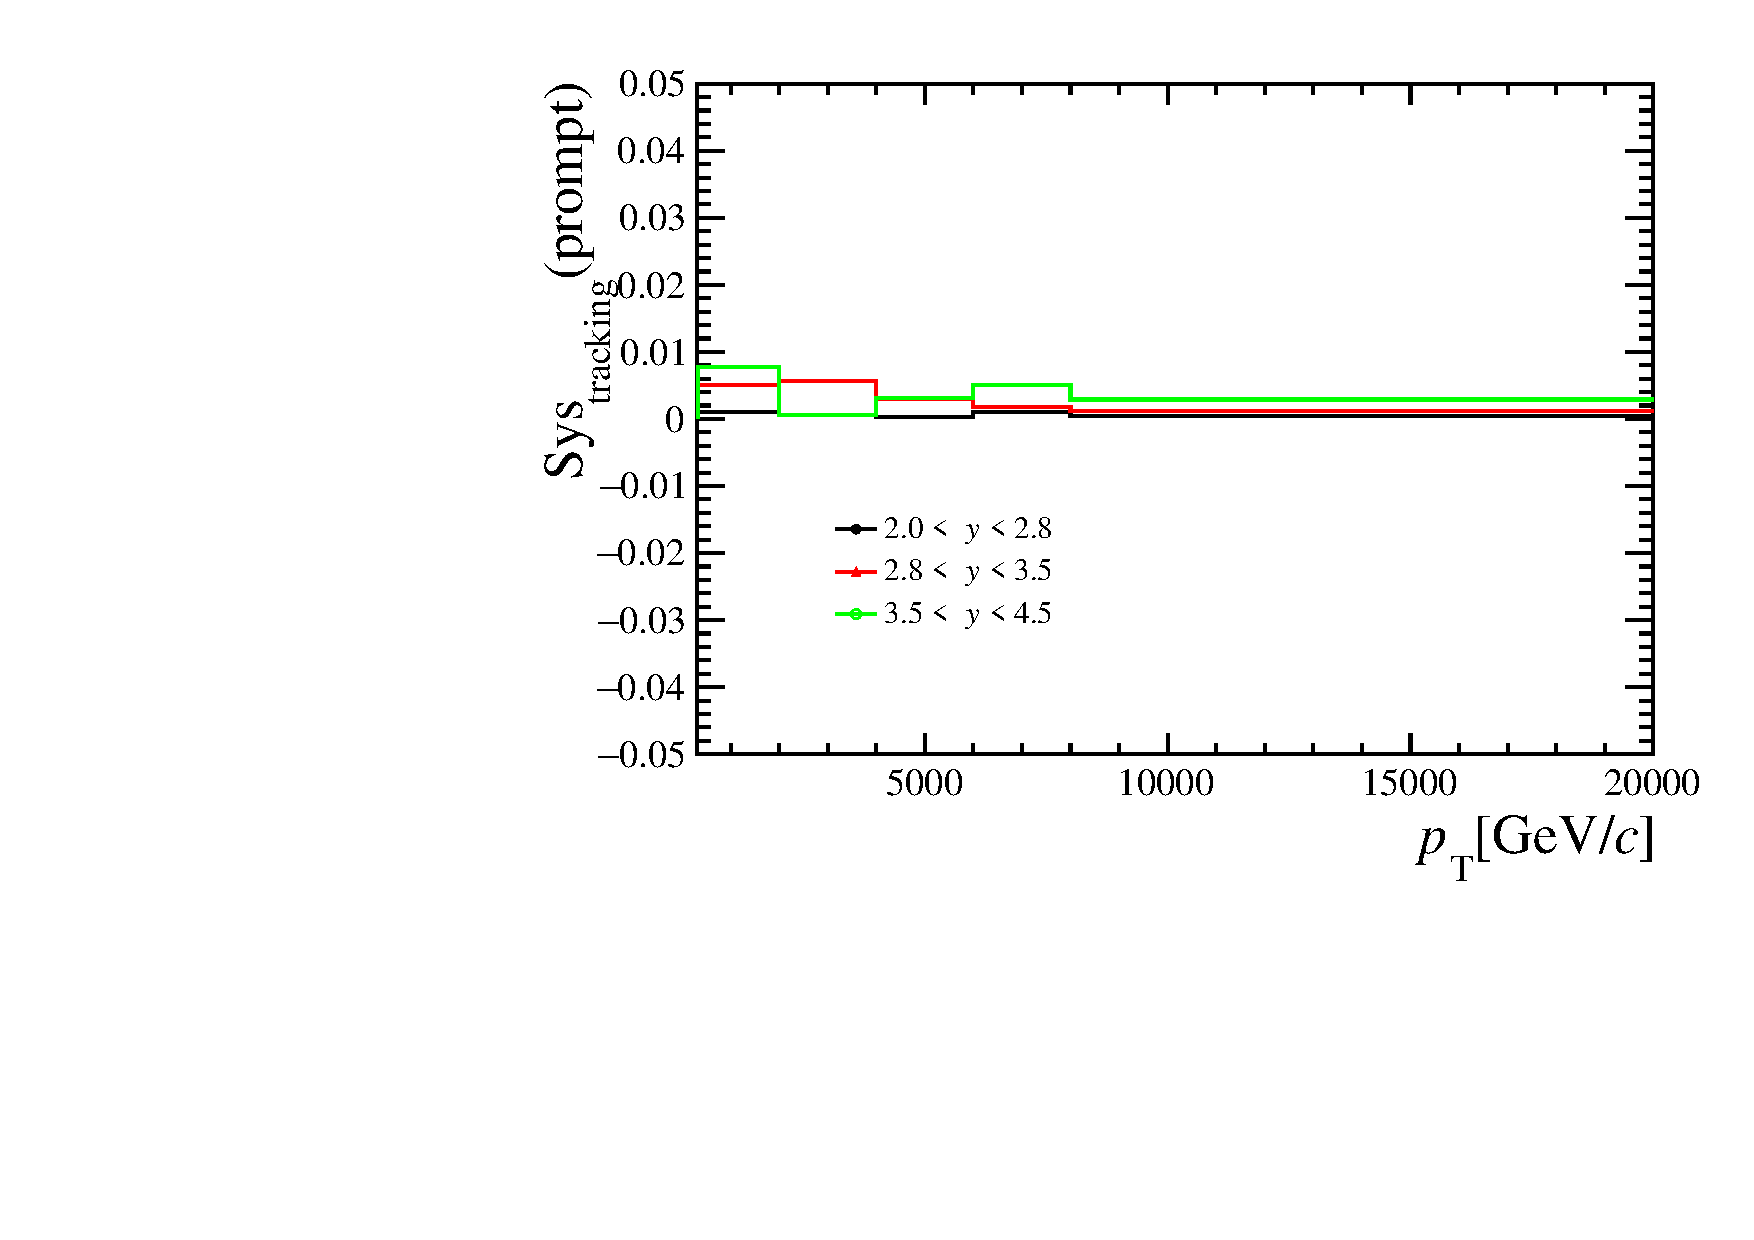
\includegraphics[width=0.49\linewidth]{pdf/SysTracking/n1Errp_point.pdf}
      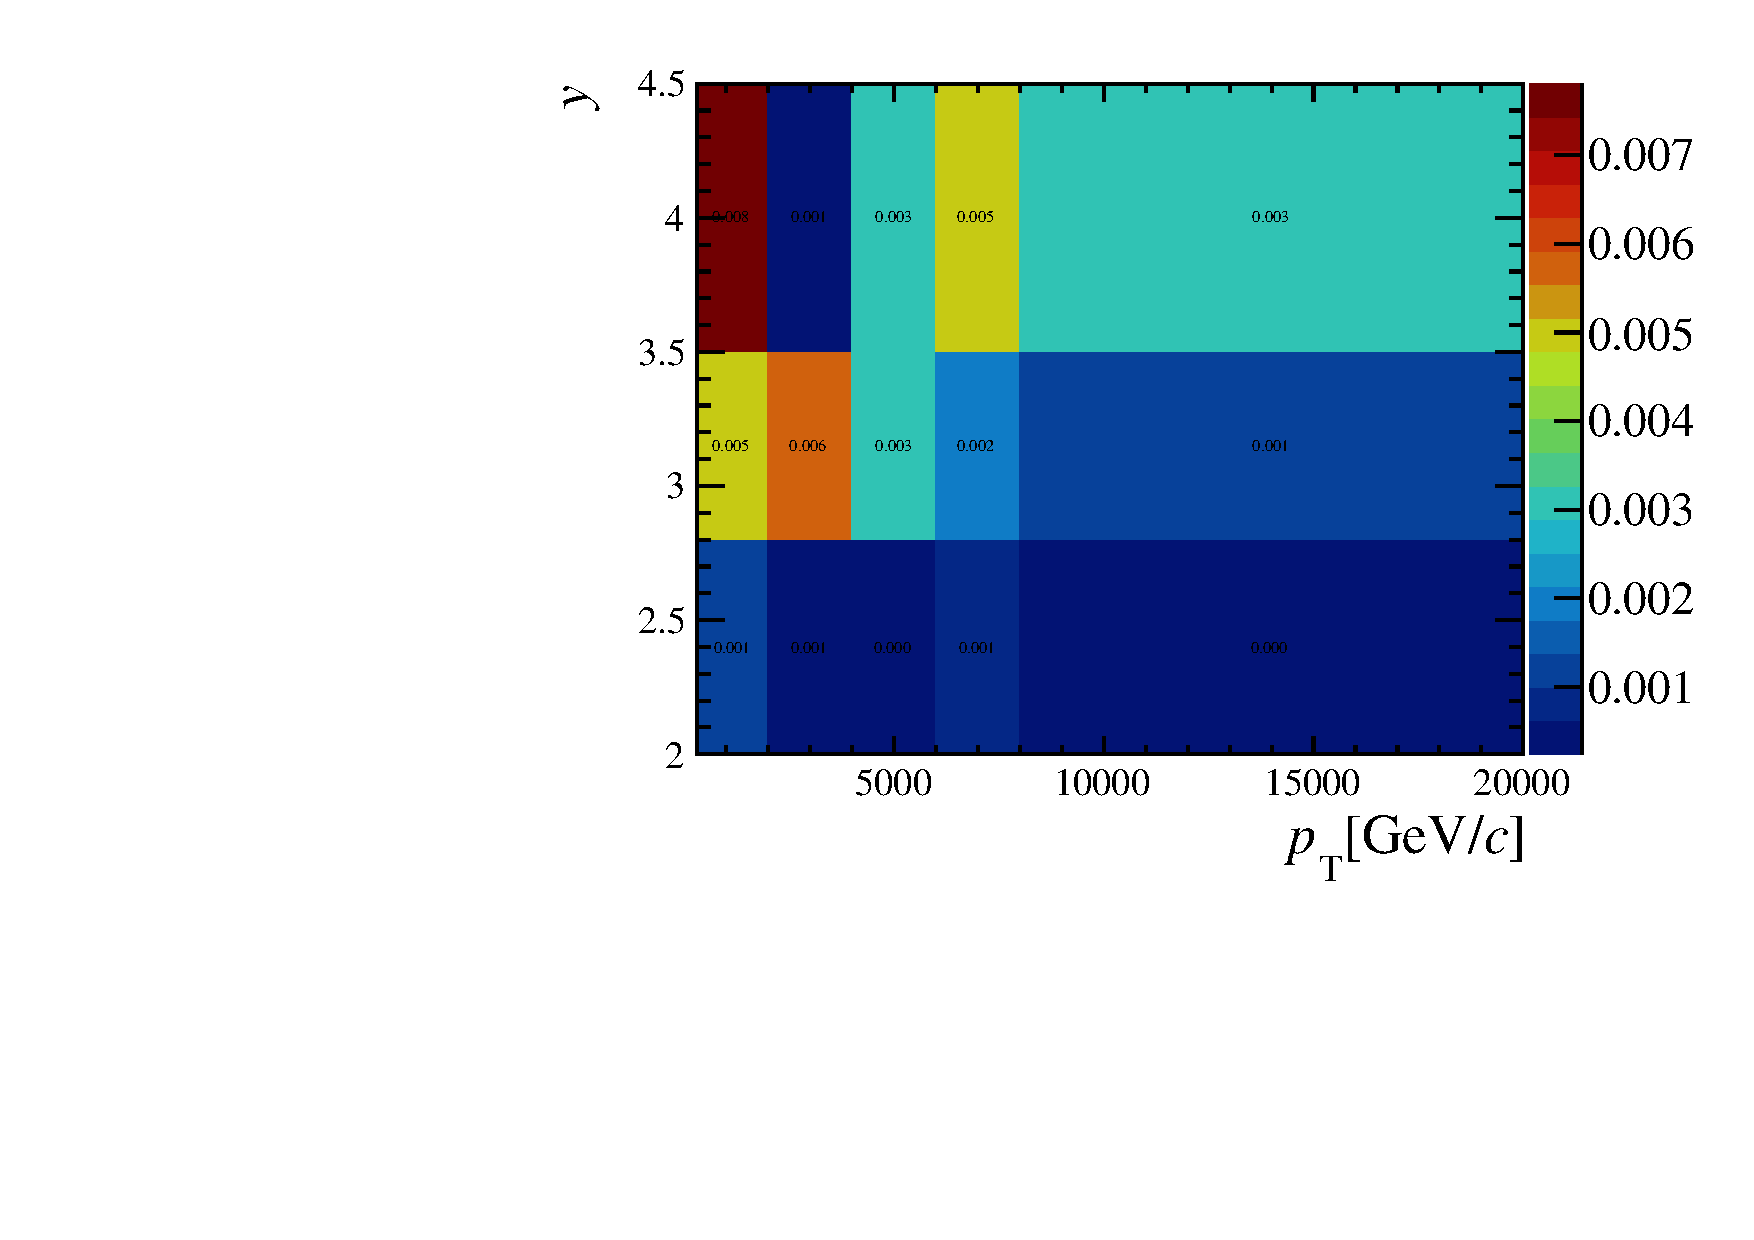
\includegraphics[width=0.49\linewidth]{pdf/SysTracking/n1Errp.pdf}
      \vspace*{-0.5cm}
      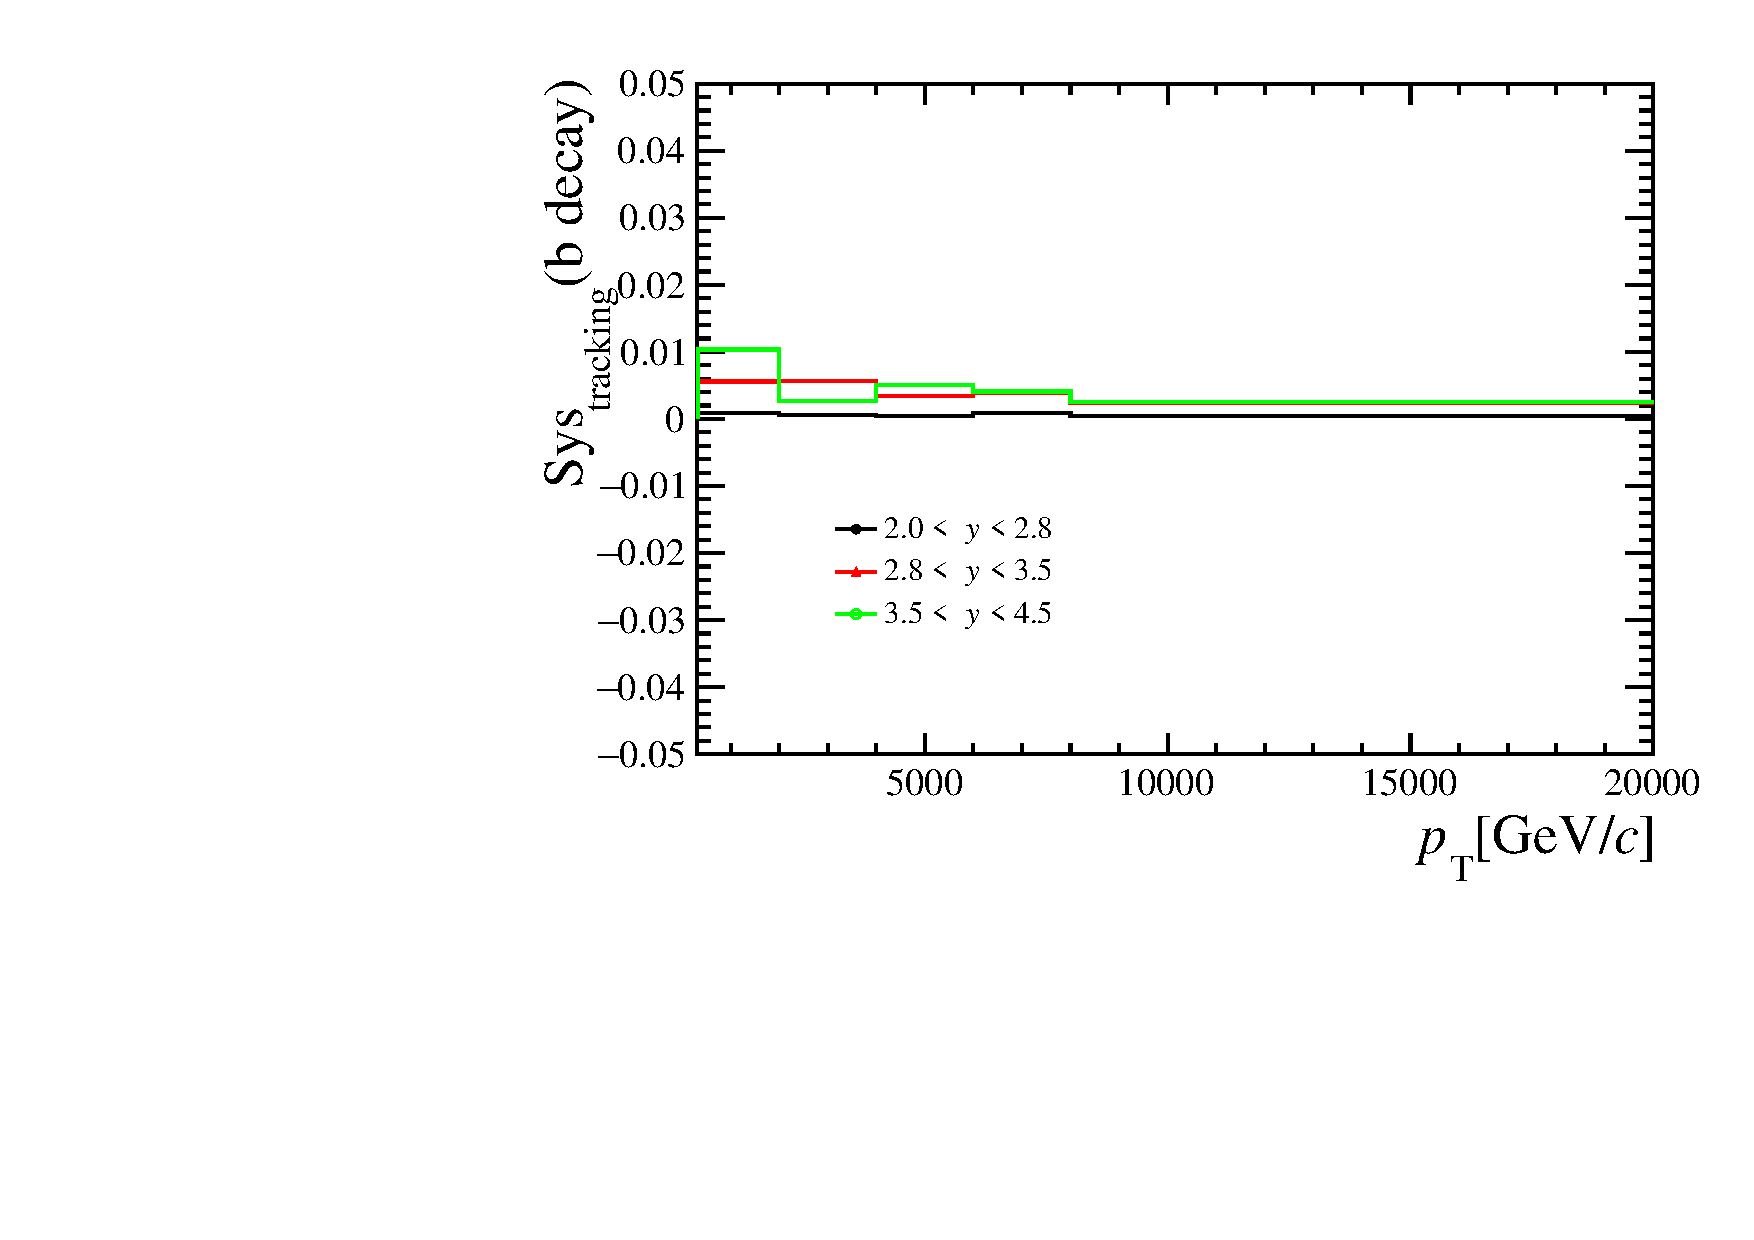
\includegraphics[width=0.49\linewidth]{pdf/SysTracking/n1Errb_point.pdf}
      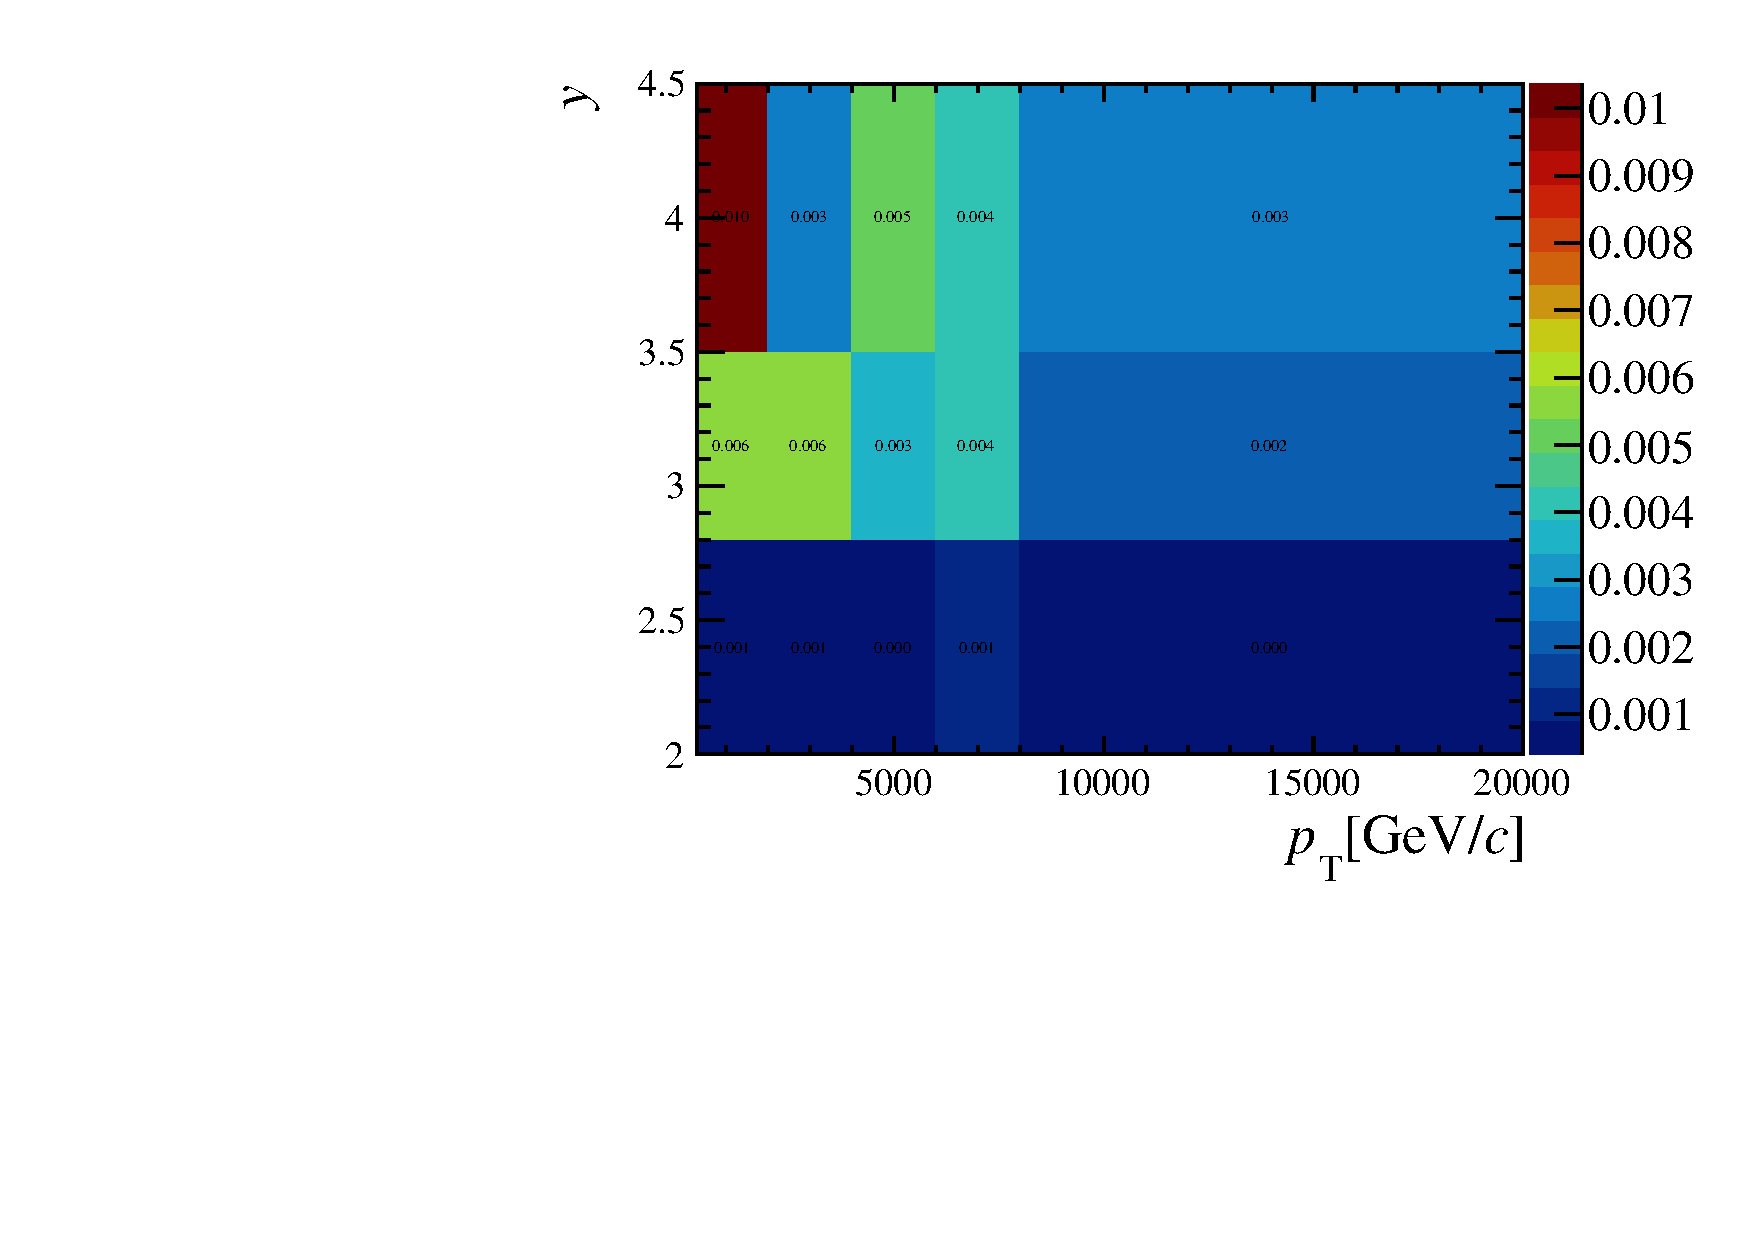
\includegraphics[width=0.49\linewidth]{pdf/SysTracking/n1Errb.pdf}
    \end{center}
    \caption{The systematic uncertainty of ratio of production due to the uncertainty of track table in each bin for PVNTRACKS from 4 to 20. The first row is that of prompt components and the second row is that of components from $b$-hadron decay.
      }
    \label{Sys_Tracking1}
\end{figure}

Another one is the choice of event multiplicity variable.
This systematic uncertainty is provided by the tracking group. 
The tracking experts indicate that the choice of the multiplicity variable (nTracks, nSPDHits, or others) is relevant for deciding the systematics.
They studied this effect and suggest $0.8\%$ per track, as detailed in Ref.~\cite{Trackweb}.
But when we calculate the ratio between \jpsi and \psitwos, the uncertainty due to the choice of multiplicity variable is canceled out since we use 
the same table for calculating both \jpsi and \psitwos.


\subsection{MuonID efficiency}
\label{sec:MuonIDCalib}
The systematic uncertainty due to MuonID includes the following contributions:
\begin{itemize}
\item The statistical uncertainty is due to the finite size of the calibration sample.
To estimate the systematic uncertainty due to the limited calibration sample size, we first generate two hundred tables of efficiencies from the original table, where the efficiency in each bin of each table is randomly sampled from a Gaussian distribution using the central value as the mean and the uncertainty as the width. 
Then, we obtain two hundred efficiency values from the generated efficiency tables, hence, we calculated two hundred productions of \jpsi and \psitwos in each \pt-y bin in different multiplicity region and their ratios.
Finally, we fit the distribution of the two hundred ratios (in a single bin and integrated region) with a Gaussian function. 
The ratio between the width and the mean value of the fitted Gaussian function is quoted as a systematic uncertainty, which is summarized in figure~\ref{Sys_PID1}.
\begin{figure}[!tbp]
    \begin{center}
      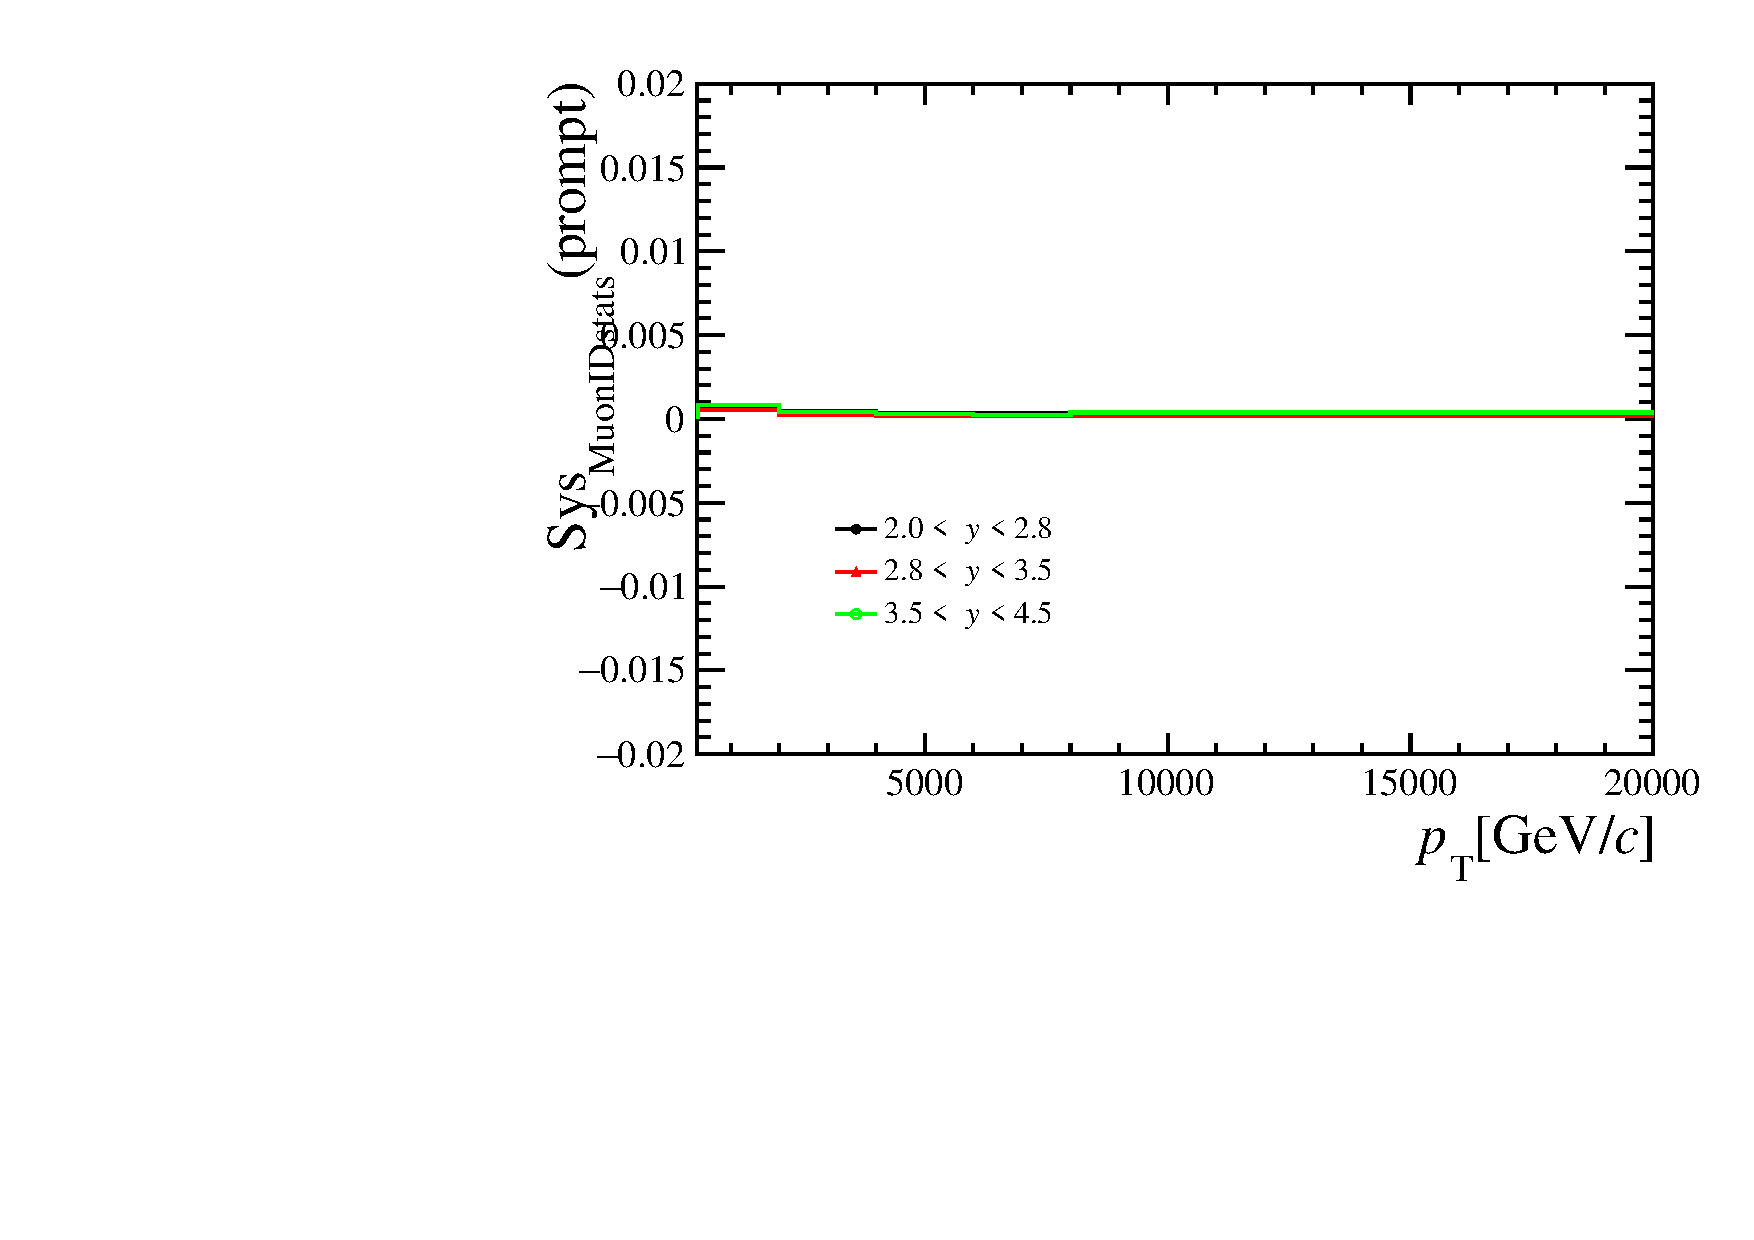
\includegraphics[width=0.49\linewidth]{pdf/SysPID/n1Errp_point.pdf}
      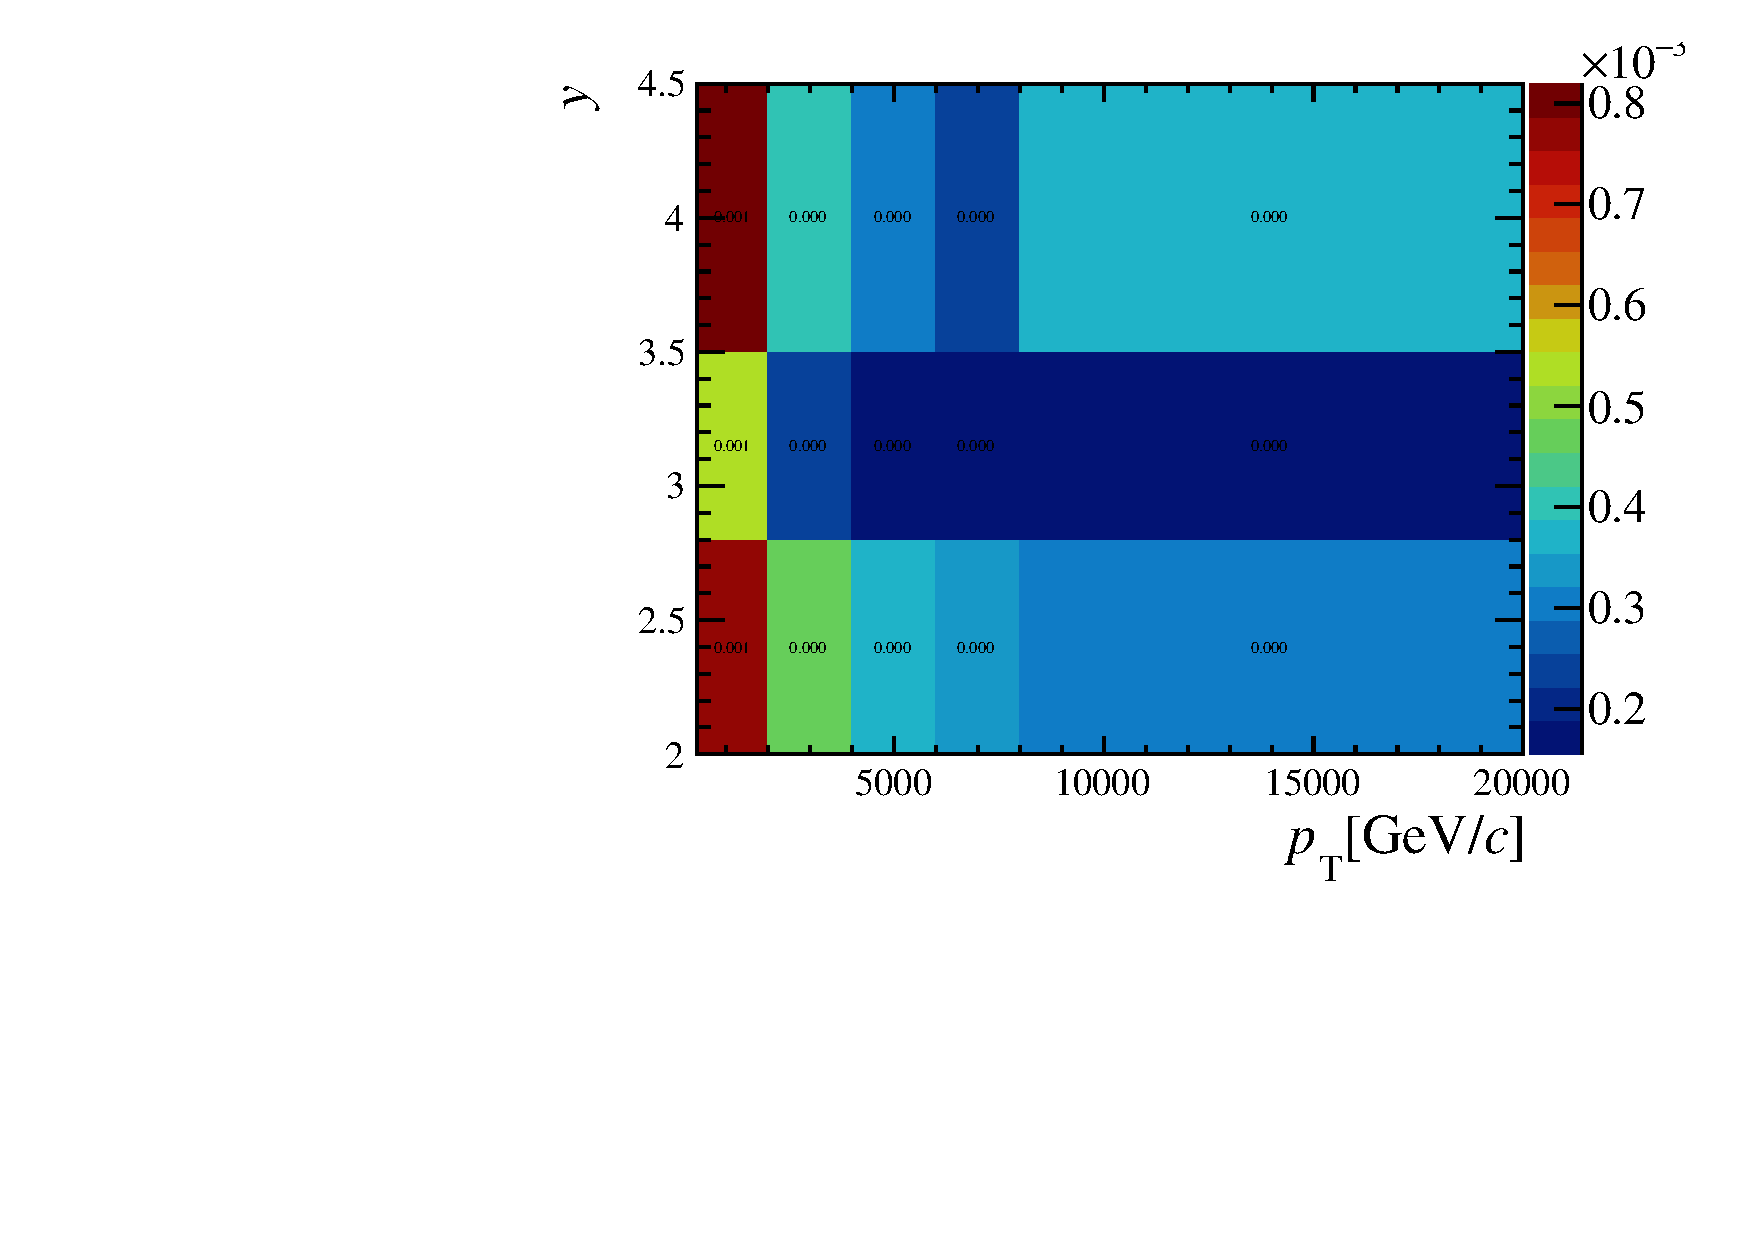
\includegraphics[width=0.49\linewidth]{pdf/SysPID/n1Errp.pdf}
      \vspace*{-0.5cm}
      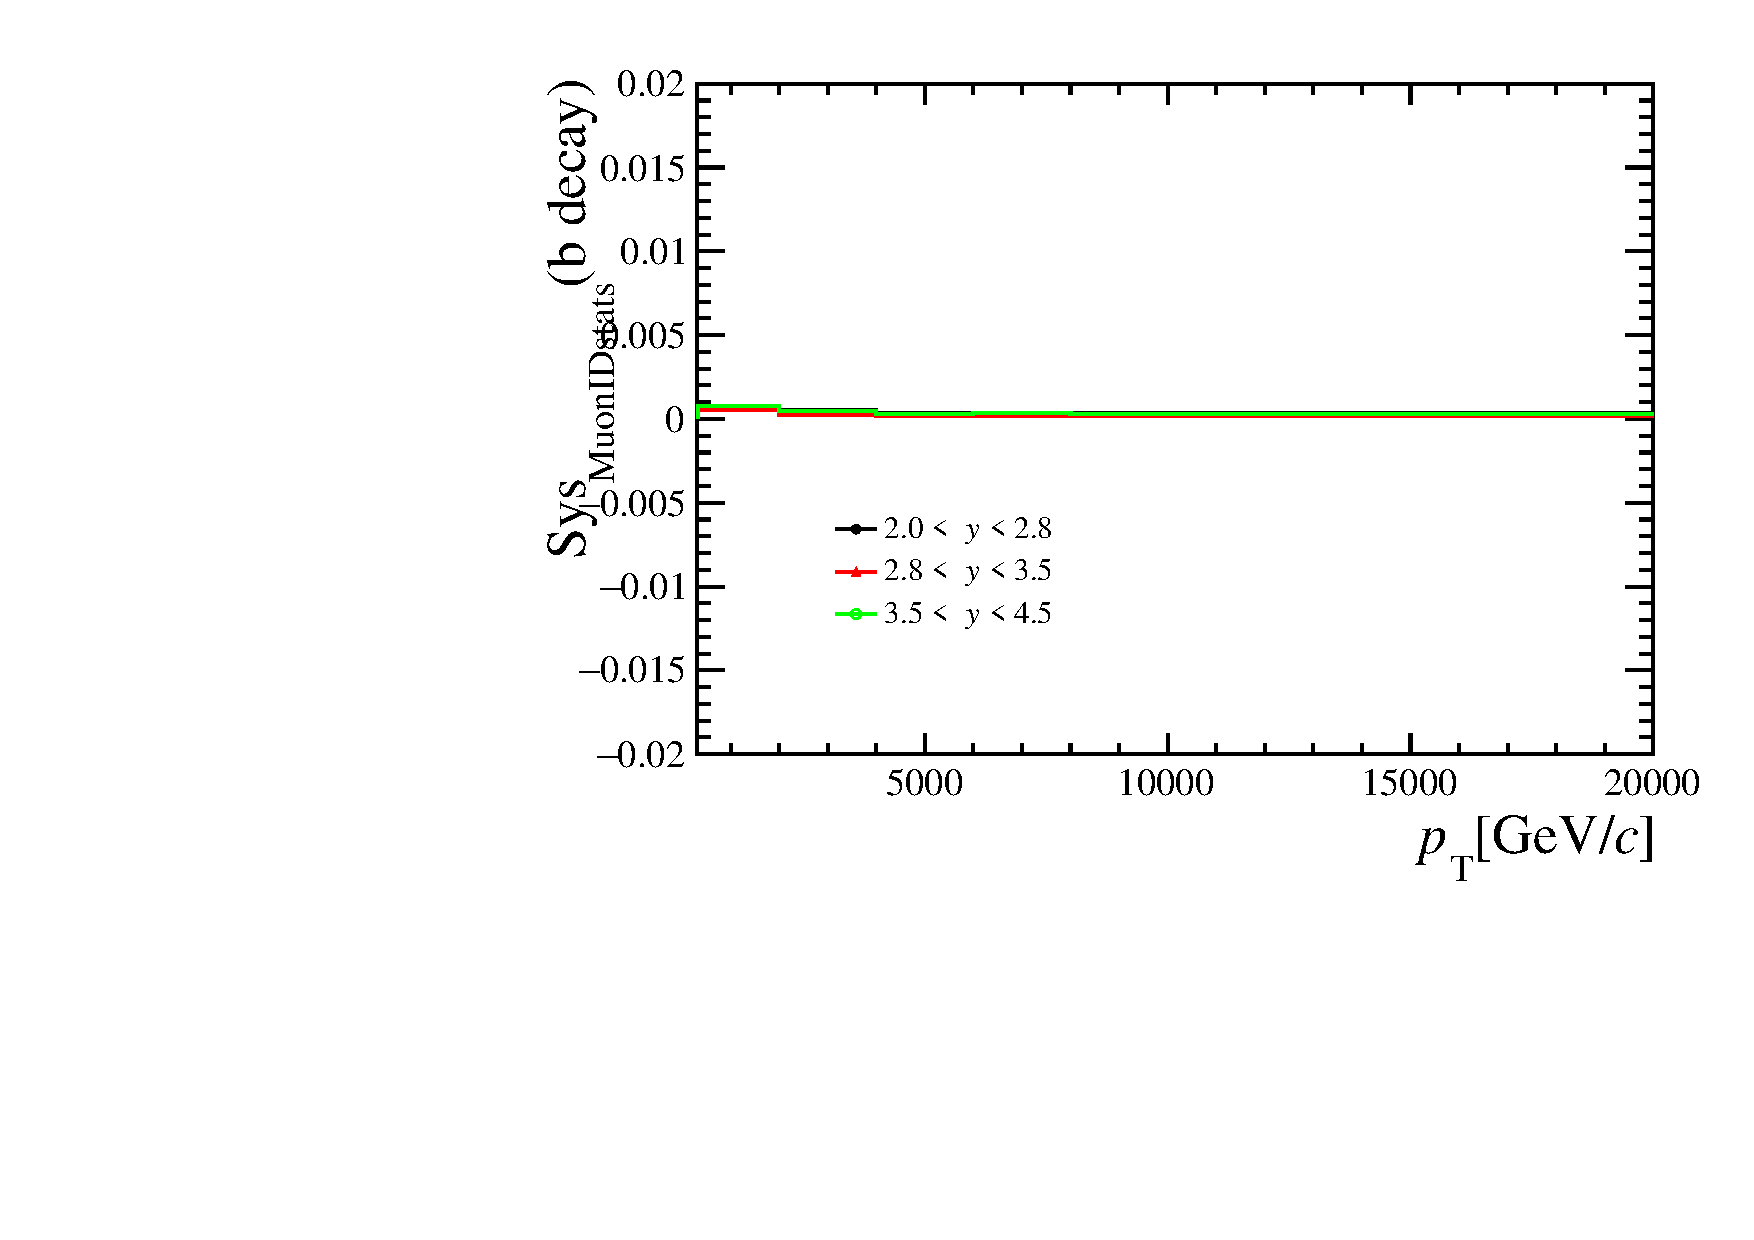
\includegraphics[width=0.49\linewidth]{pdf/SysPID/n1Errb_point.pdf}
      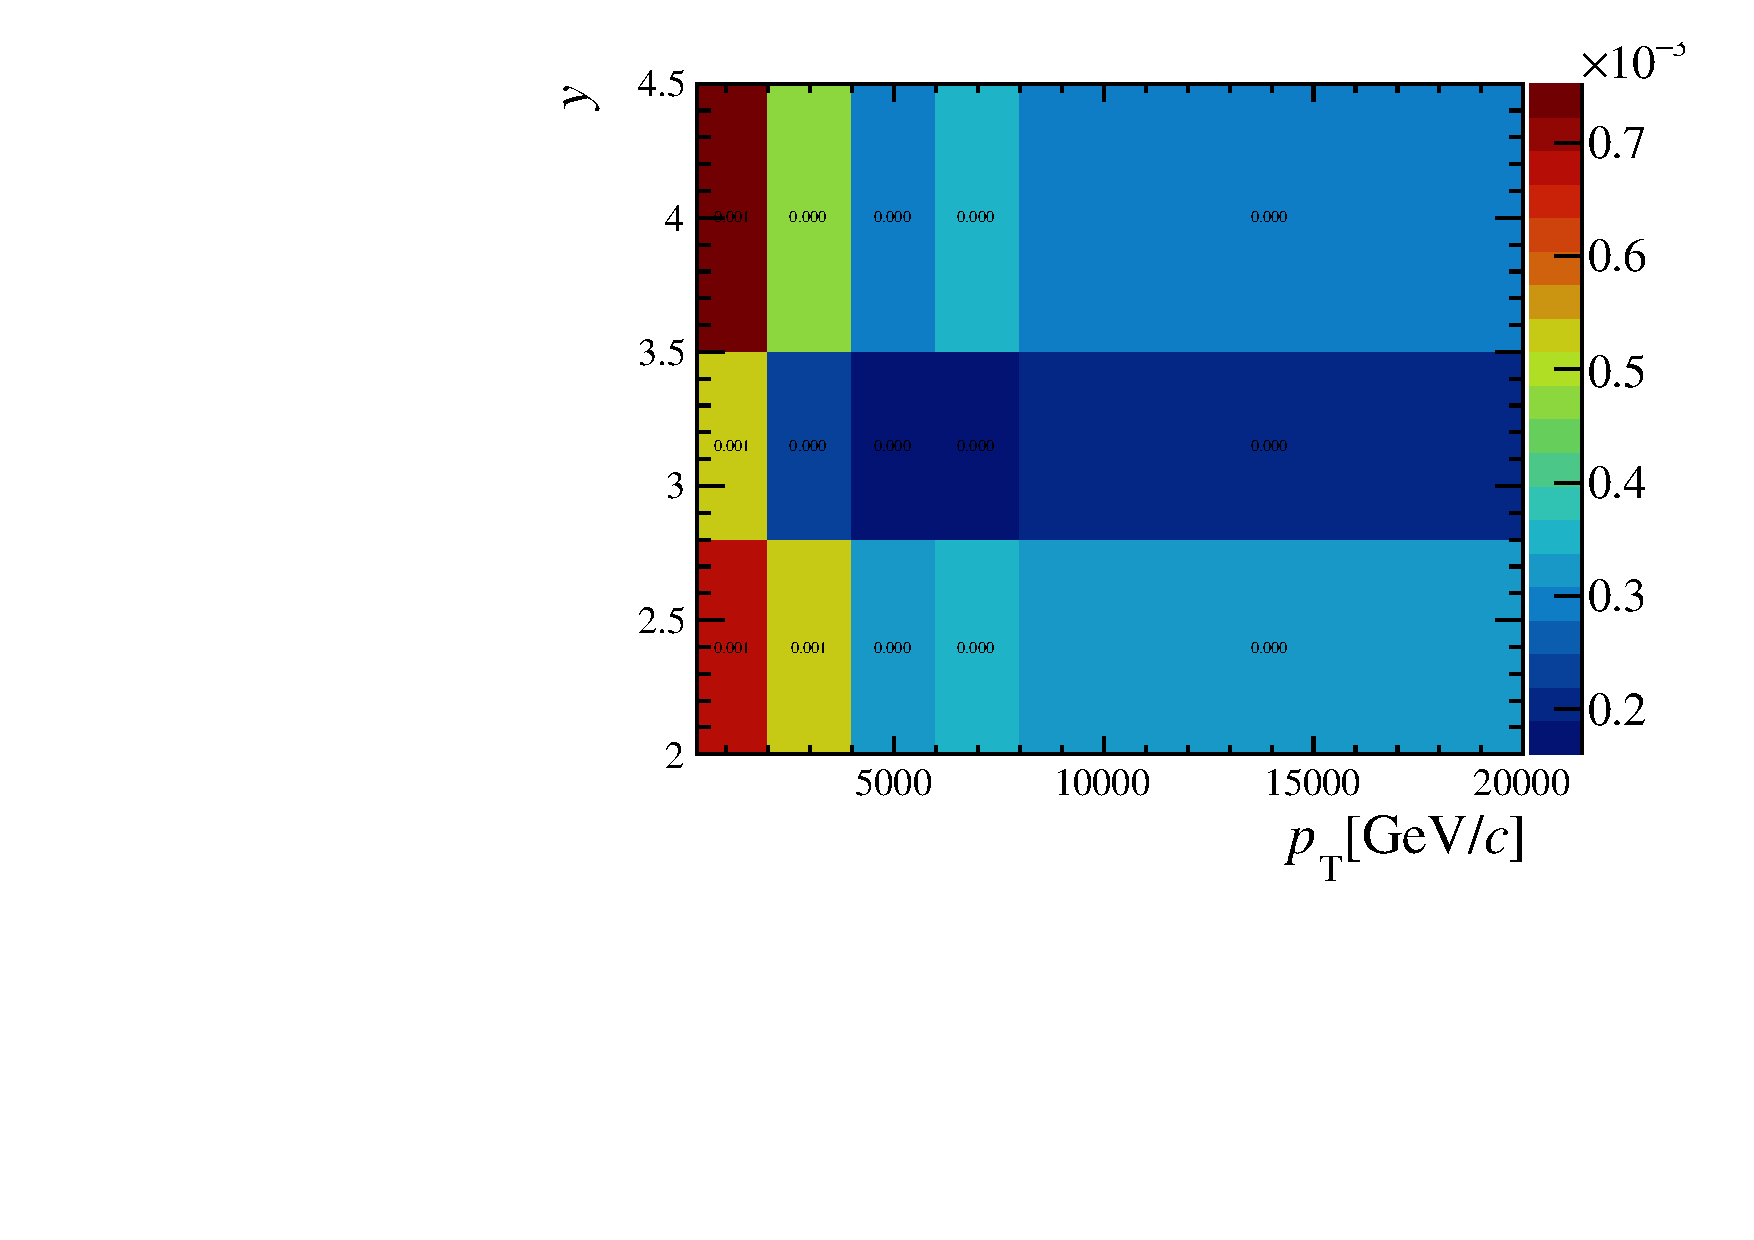
\includegraphics[width=0.49\linewidth]{pdf/SysPID/n1Errb.pdf}
    \end{center}
    \caption{The systematic uncertainty of ratio of production due to the statistical uncertainty of PID efficiency in each bin for PVNTRACKS from 4 to 20. The first row is that of prompt components and the second row is that of components from $b$-hadron decay.
      }
    \label{Sys_PID1}
\end{figure}
% \begin{table}[h]
%     \centering
%     \caption{Summary of systematic uncertainties of ratio of integrated production due to the uncertainty of PID table for PVNTRACKS from 4 to 20.}
% \begin{center}
%     \begin{tabular}{ c | c | c }
%         \hline
%         Region & prompt (\%) & from $b$ (\%)\\
%         \hline
%         2.0$<$y$<$2.8&0.05&0.05\\
%         2.8$<$y$<$3.5&0.04&0.03\\
%         3.5$<$y$<$4.5&0.06&0.06\\
%         \hline
%         0\gevc $<$\pt$<$2\gevc&0.05&0.05\\
%         2\gevc $<$\pt$<$4\gevc&0.03&0.03\\
%         4\gevc $<$\pt$<$6\gevc&0.02&0.02\\
%         6\gevc $<$\pt$<$8\gevc&0.02&0.02\\
%         8\gevc $<$\pt$<$20\gevc&0.02&0.02\\
%         \hline
%         all \pt-y region&0.03&0.03\\
%         \hline
%     \end{tabular}
% \end{center}
% \label{Sys_PID1_int}
% \end{table}
\item Uncertainty due to binning scheme of the calibration sample, studied by varying the binning method in $p_\mu$, $\eta_\mu$, and nSPDHits respectively.
The default one and the two alternative binning schemes could be found below.
The nominal binning scheme of the muon ID efficiency for muons we use to calculate the muon ID efficiency of \jpsi and \psitwos mesons is defined:
\begin{itemize}
  \item $p_\mu$ boundaries [\gevc]: 3, 6, 8, 10, 12, 13, 14, 15, 16, 18, 20, 24, 28, 32, 40, 60, 70, 80, 90, 100, 200, 1000
  \item $\eta$ boundaries: 2.0, 2.5, 3.0, 3.5, 4.0, 4.5, 4.9
  \item nSPDhits boundaries: 0, 200, 400, 1000.
\end{itemize}

One of the two alternative binning schemes is defined:
\begin{itemize}
  \item $p_\mu$ boundaries [\gevc]: 5, 7, 9, 11, 12, 13, 14, 15, 17, 19, 23, 27, 32, 40, 55, 65, 75, 85, 95, 150, 200, 1000
  \item $\eta$ boundaries: 2.0, 2.4, 2.9, 3.4, 3.9, 4.4, 4.9
  \item nSPDhits boundaries: 0, 300, 500, 1000.
\end{itemize}

The other one binning schemes is defined:
\begin{itemize}
  \item $p_\mu$ boundaries [\gevc]: 3, 5.5, 7.5, 9.5, 11.5, 12.5, 13.5, 14.5, 15.5, 17.5, 19.5, 23.5, 27.5, 32, 38, 48, 58, 68, 78, 88, 98, 198,1000
  \item $\eta$ boundaries: 2.0, 2.6, 3.1, 3.6, 4.1, 4.6, 4.9
  \item nSPDhits boundaries: 0, 150, 480, 1000.
\end{itemize}
The maximum difference between the two new ratios calculated by new efficiency and the original ratio is quoted as the systematic uncertainty.
The relative uncertainties for the ratio in each bin for PVNTRACKS from 4 to 20 are summarized in Fig~\ref{Sys_PID2}.
\begin{figure}[!tbp]
    \begin{center}
      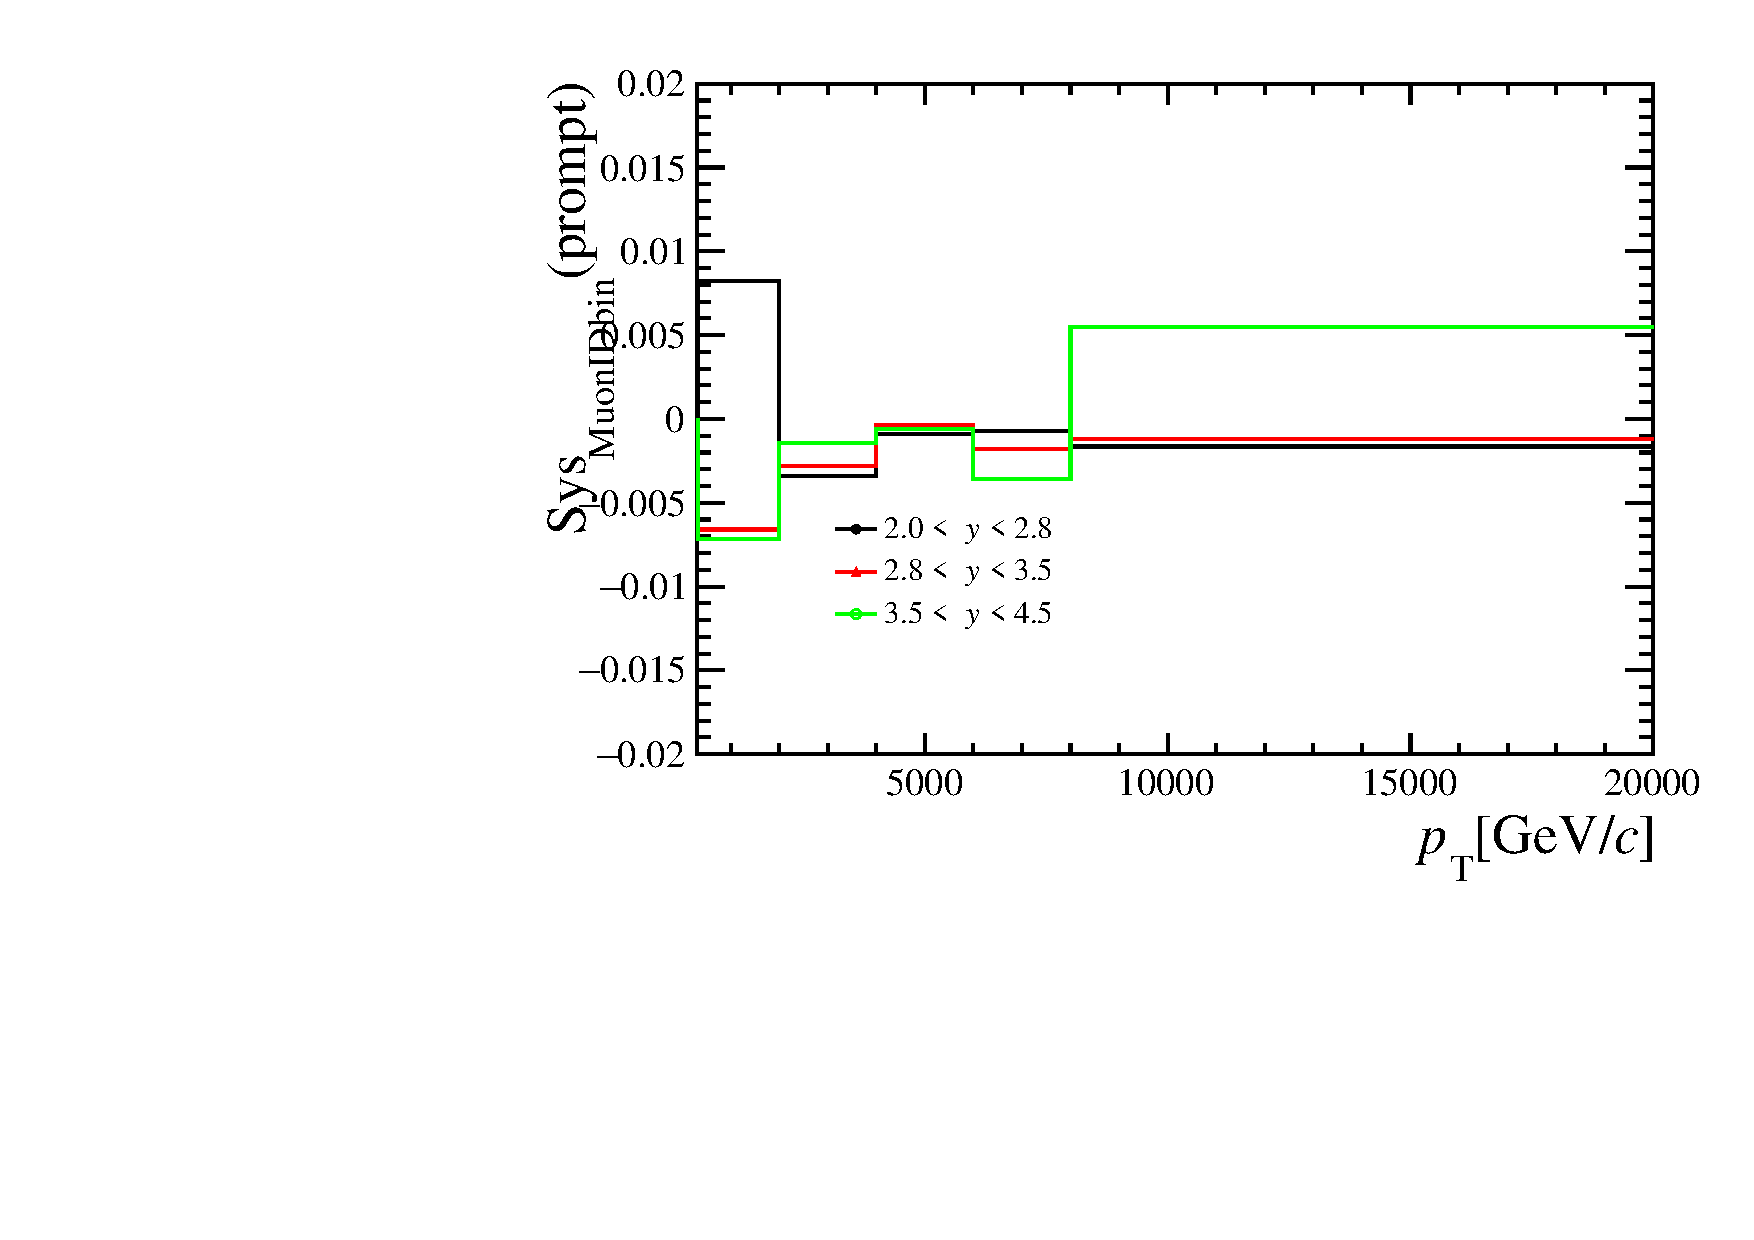
\includegraphics[width=0.49\linewidth]{pdf/SysPID/n1InBinErrp_point.pdf}
      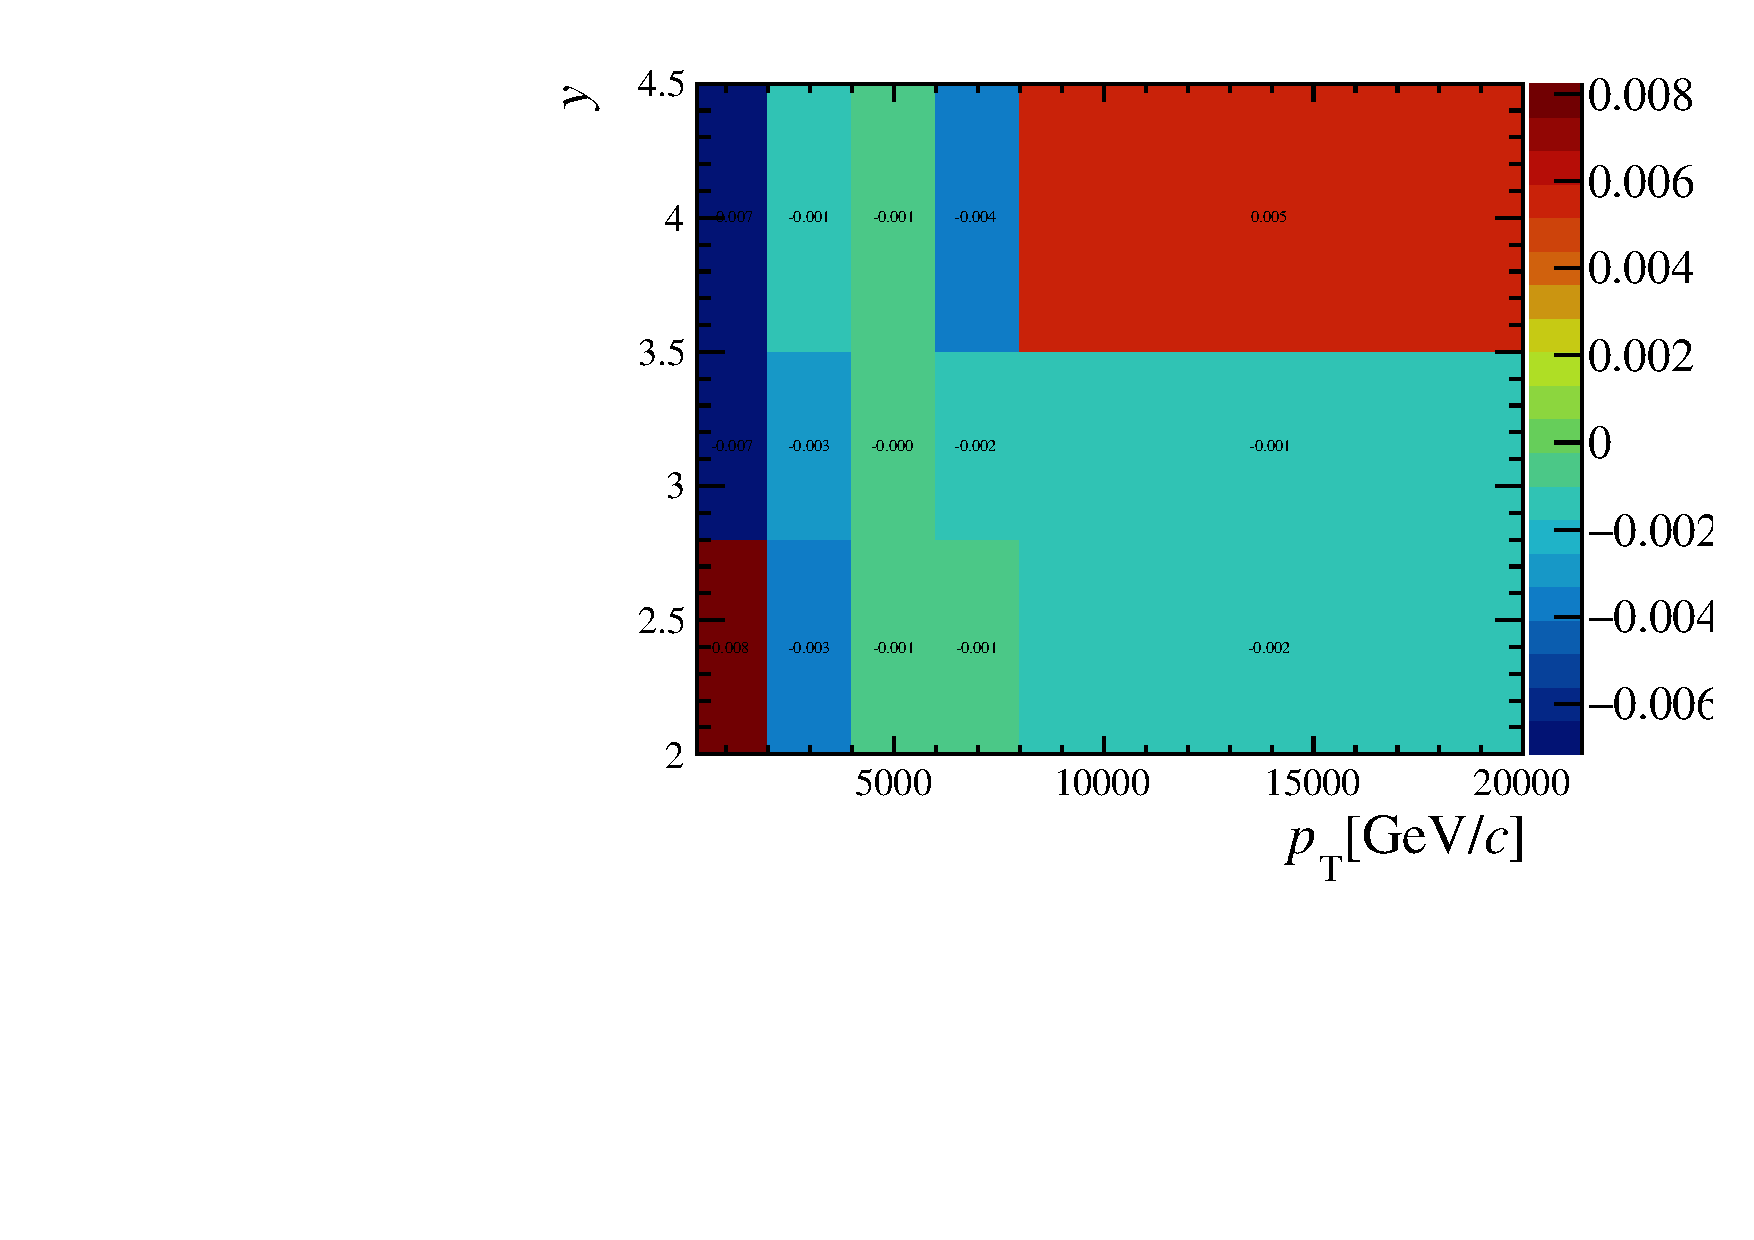
\includegraphics[width=0.49\linewidth]{pdf/SysPID/n1InBinErrp.pdf}
      \vspace*{-0.5cm}
      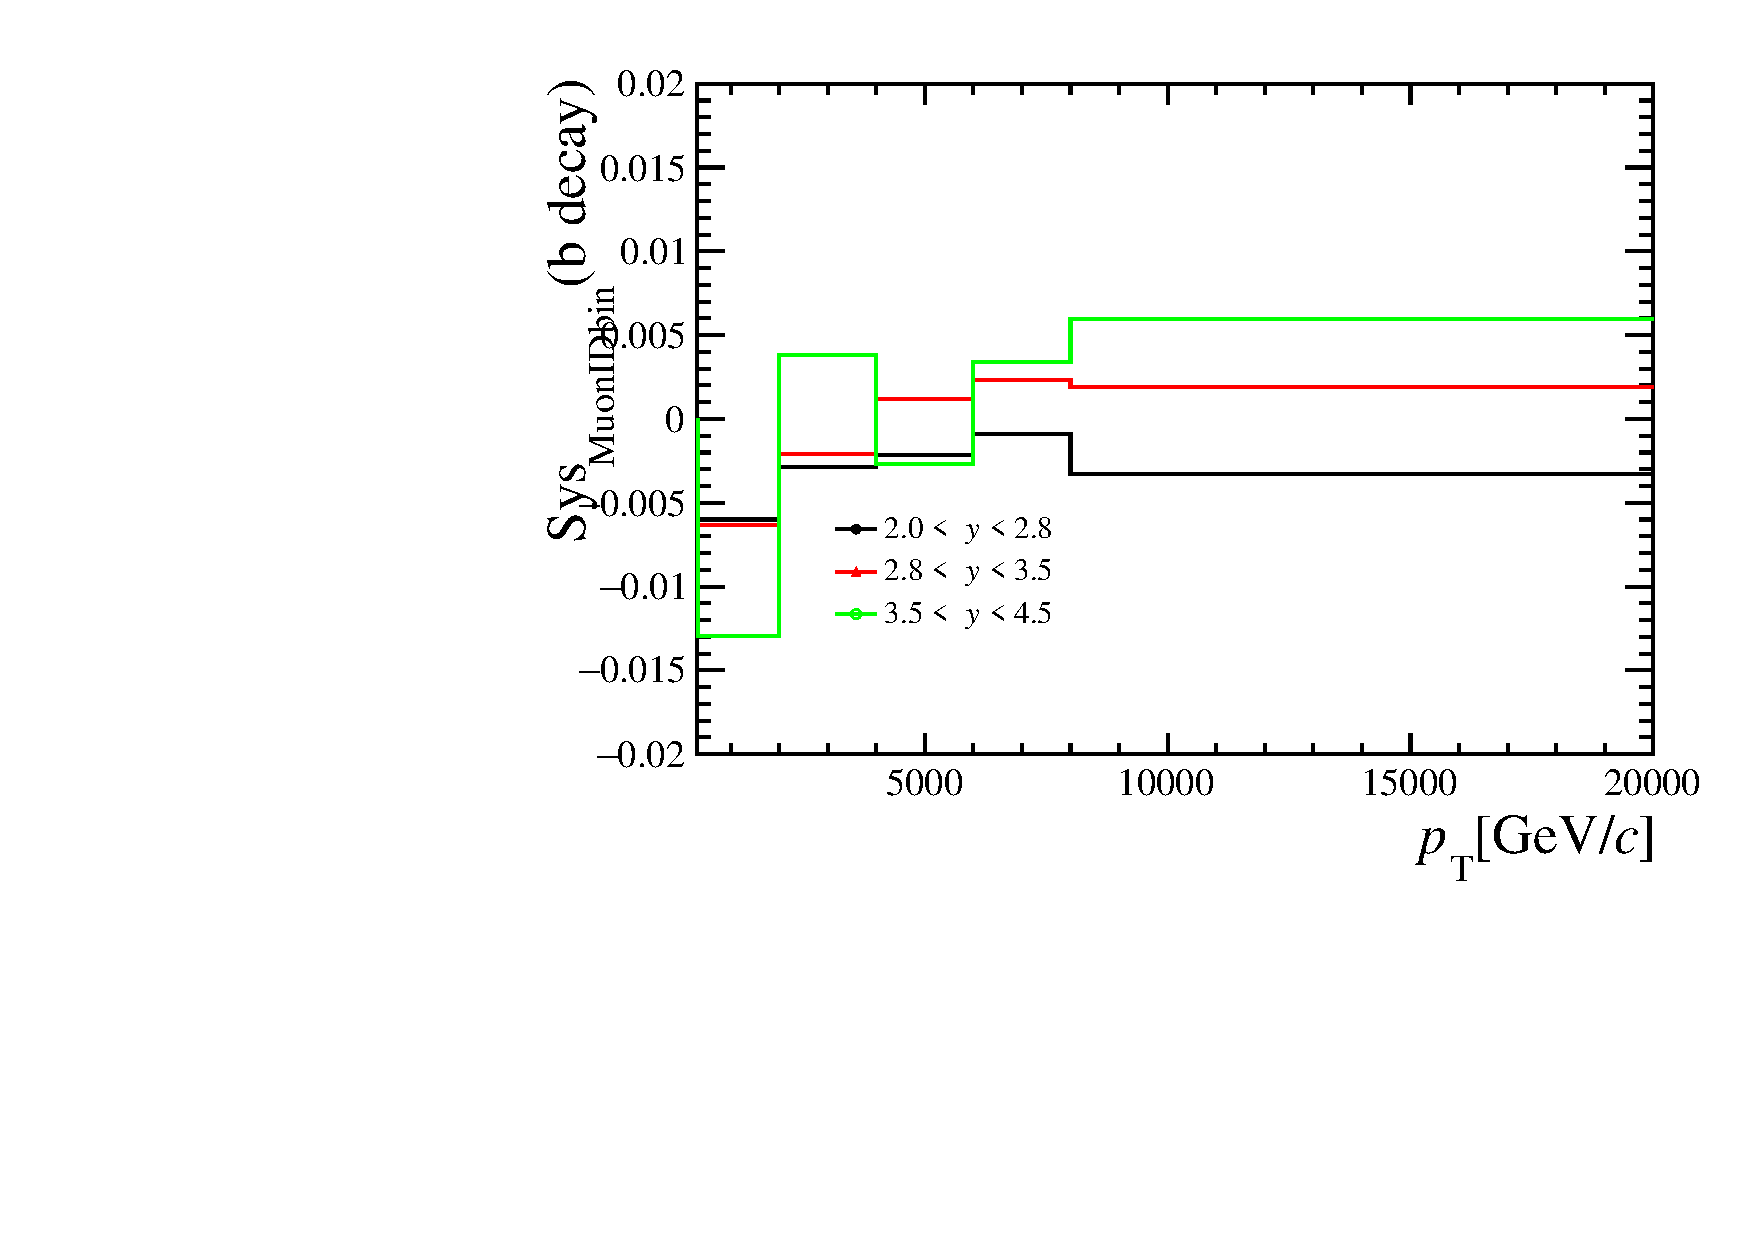
\includegraphics[width=0.49\linewidth]{pdf/SysPID/n1InBinErrb_point.pdf}
      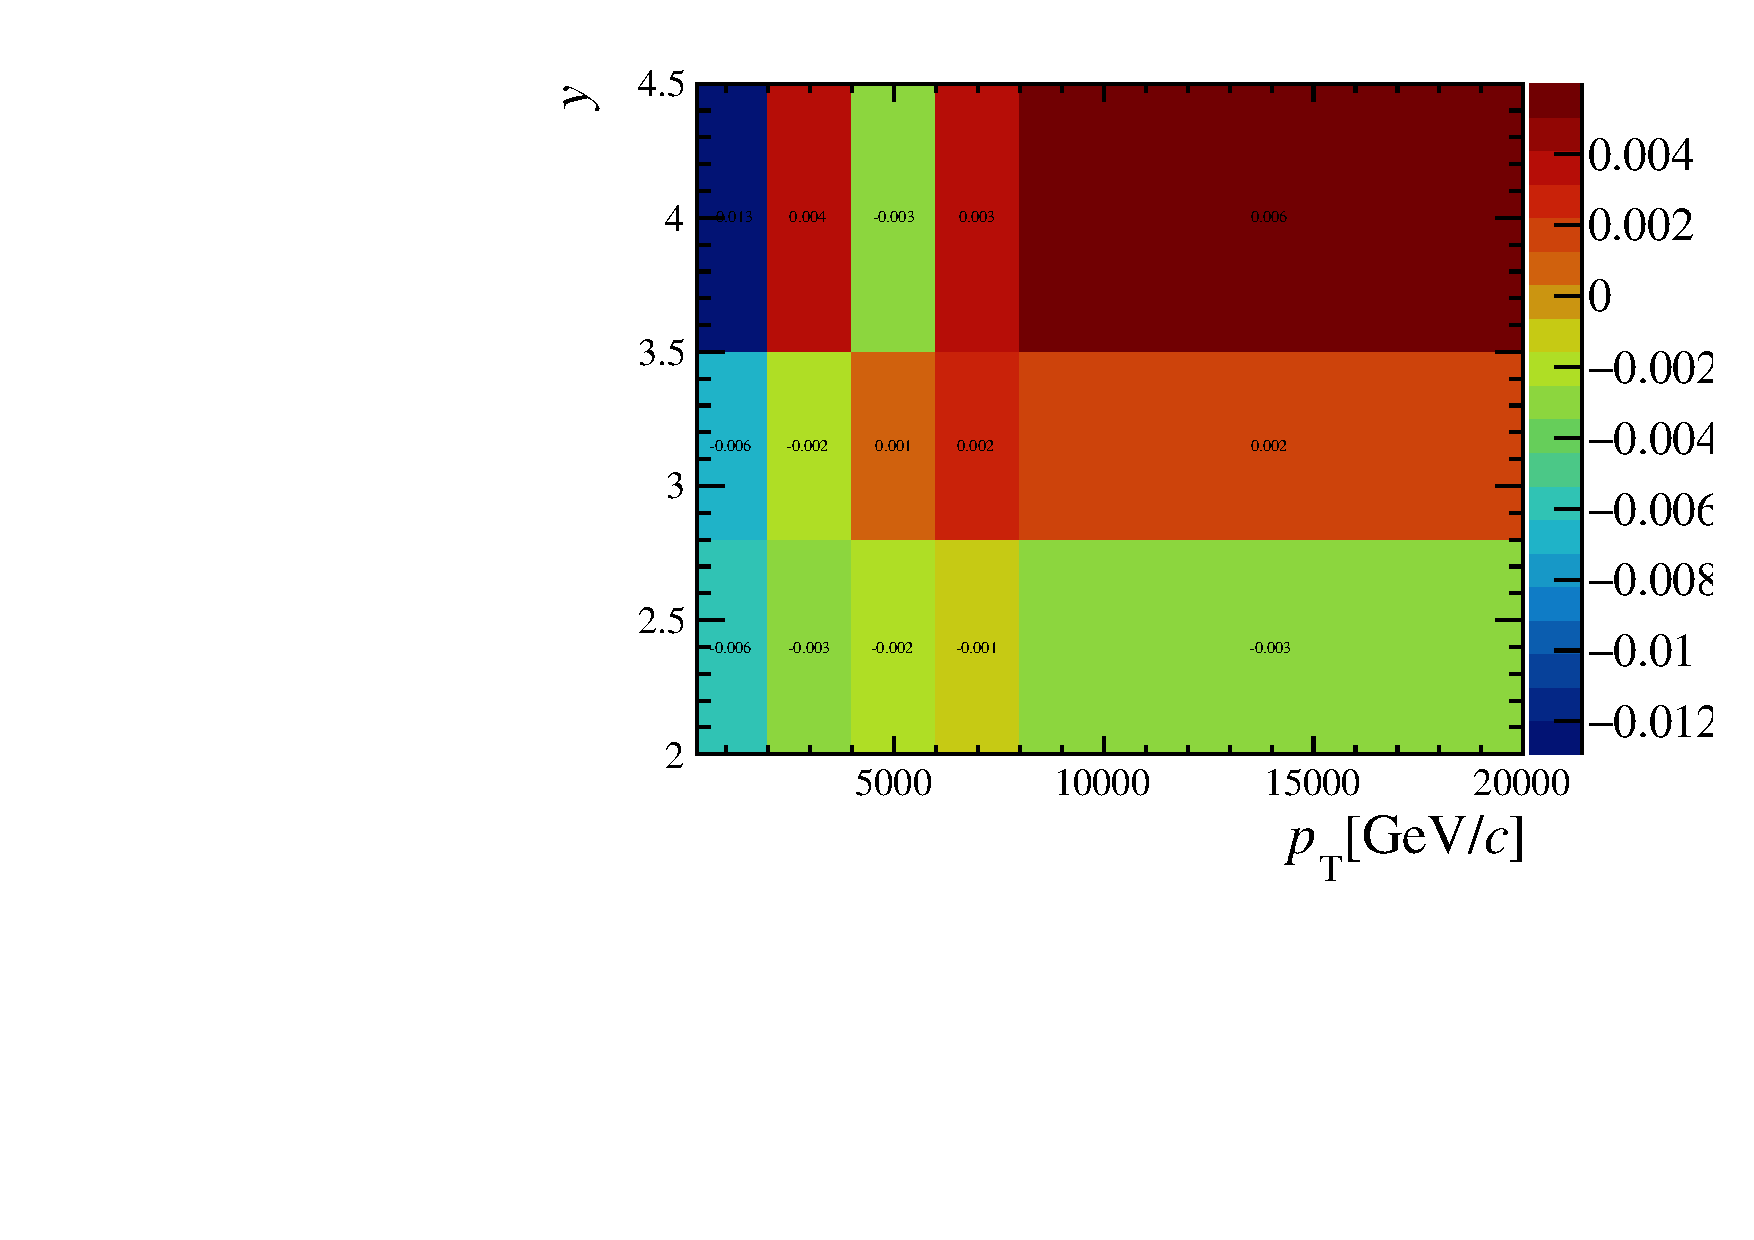
\includegraphics[width=0.49\linewidth]{pdf/SysPID/n1InBinErrb.pdf}
    \end{center}
    \caption{The systematic uncertainty of ratio of production due to the binning scheme of calibration sample in each bin for PVNTRACKS from 4 to 20. The first row is that of prompt components and the second row is that of components from $b$-hadron decay.
      }
    \label{Sys_PID2}
\end{figure}
\end{itemize}

\subsection{MC sample size}
\label{sec:MCSize}
The limited size of the simulation sample used to determine the efficiencies is a source of systematic uncertainties. 
The uncertainty of ratio due to MC sample size in different bin for PVNTRACKS from 4 to 20 are 
summarized in Fig~\ref{Sys_MCSize}.
\begin{figure}[!tbp]
    \begin{center}
      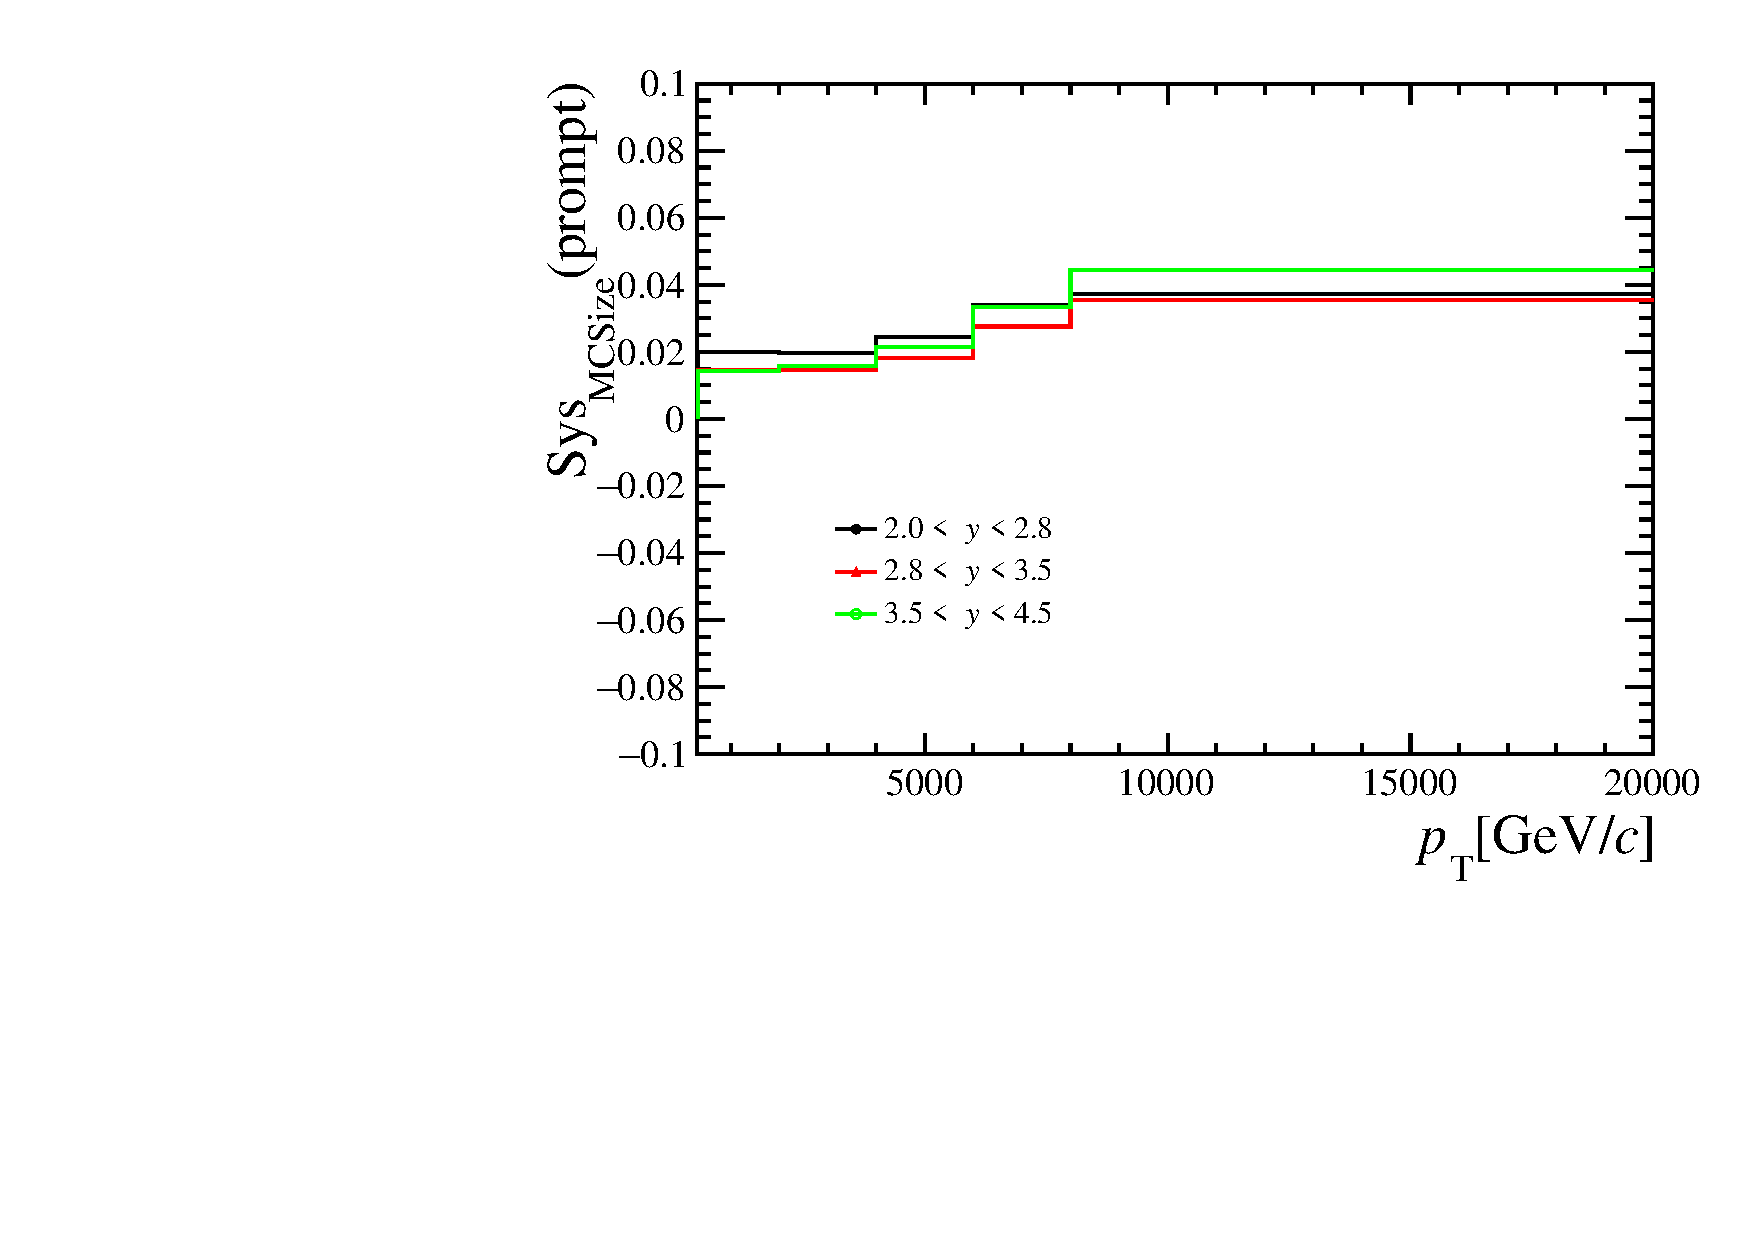
\includegraphics[width=0.49\linewidth]{pdf/SysMCSize/n1Errp_point.pdf}
      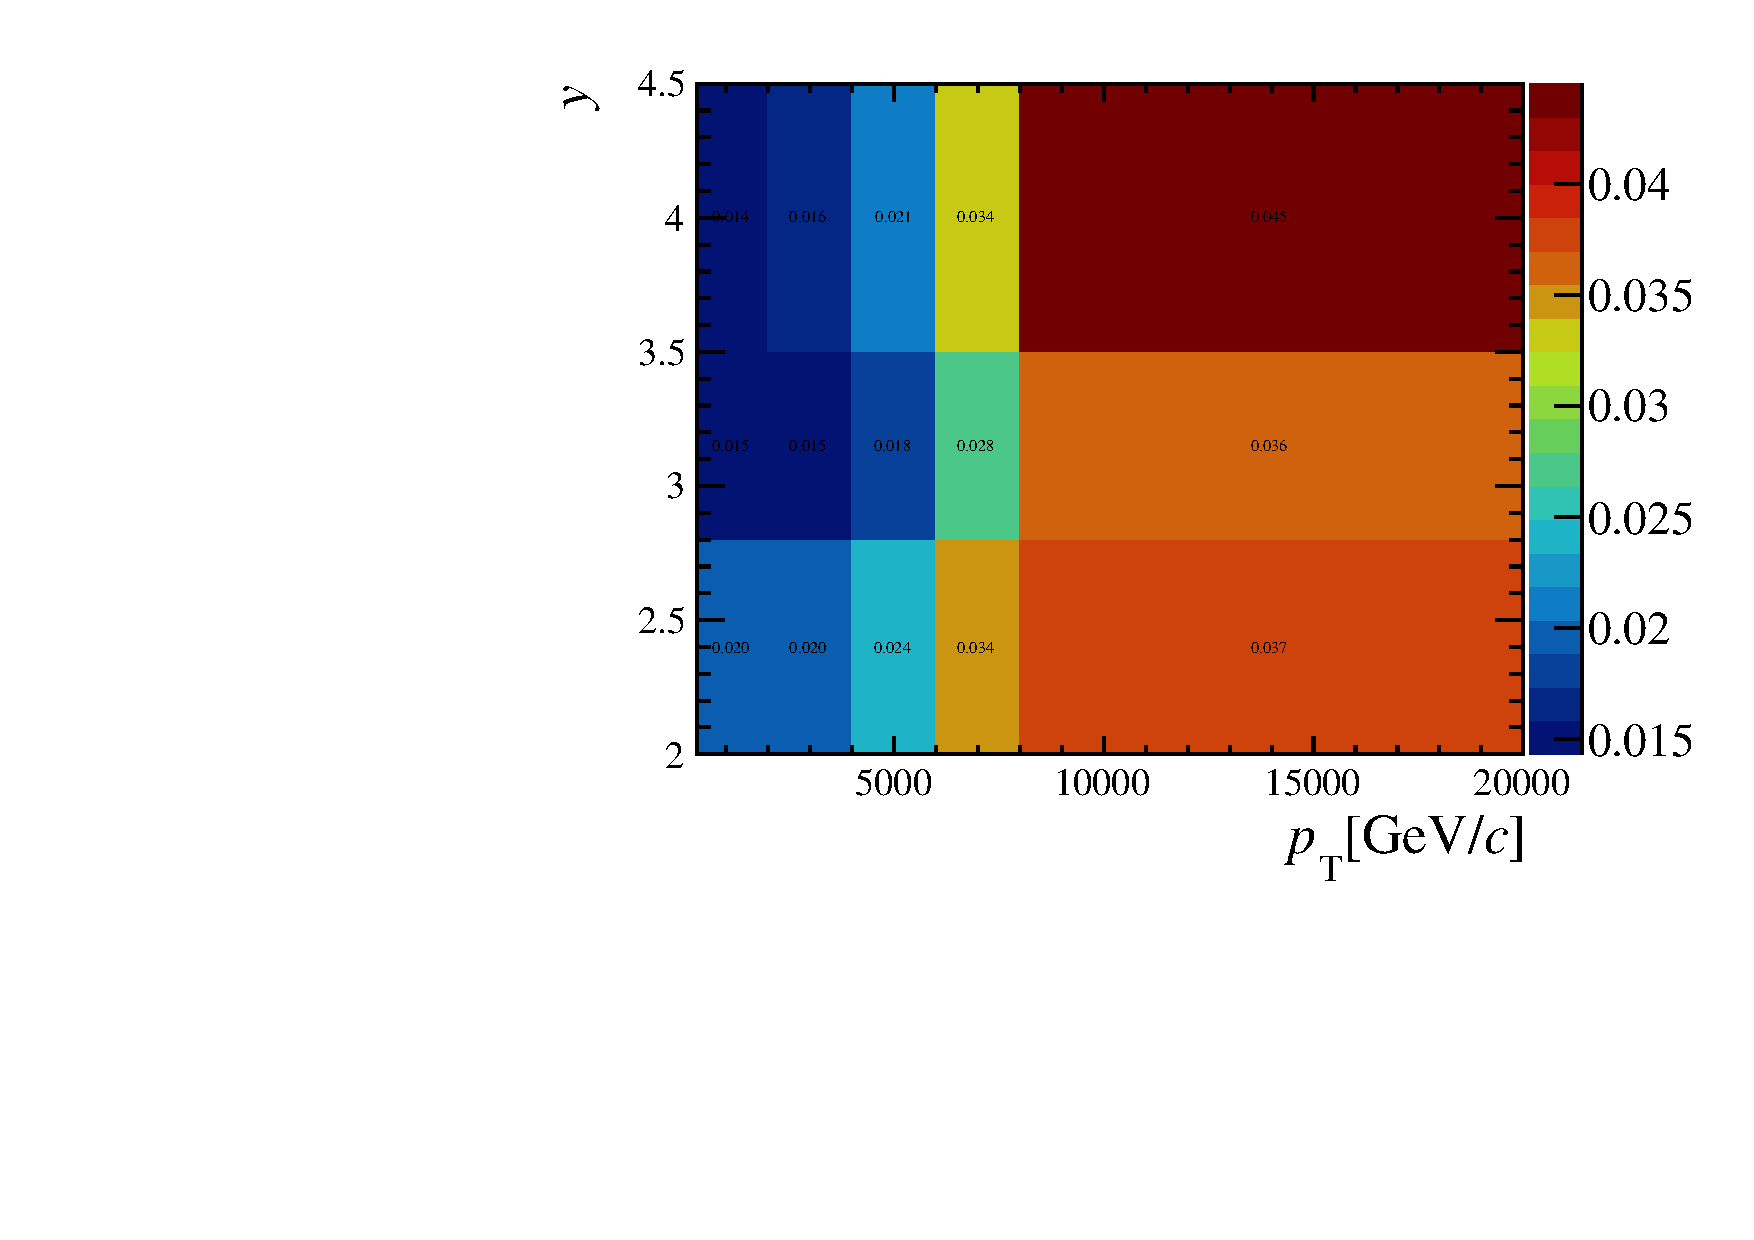
\includegraphics[width=0.49\linewidth]{pdf/SysMCSize/n1Errp.pdf}
      \vspace*{-0.5cm}
      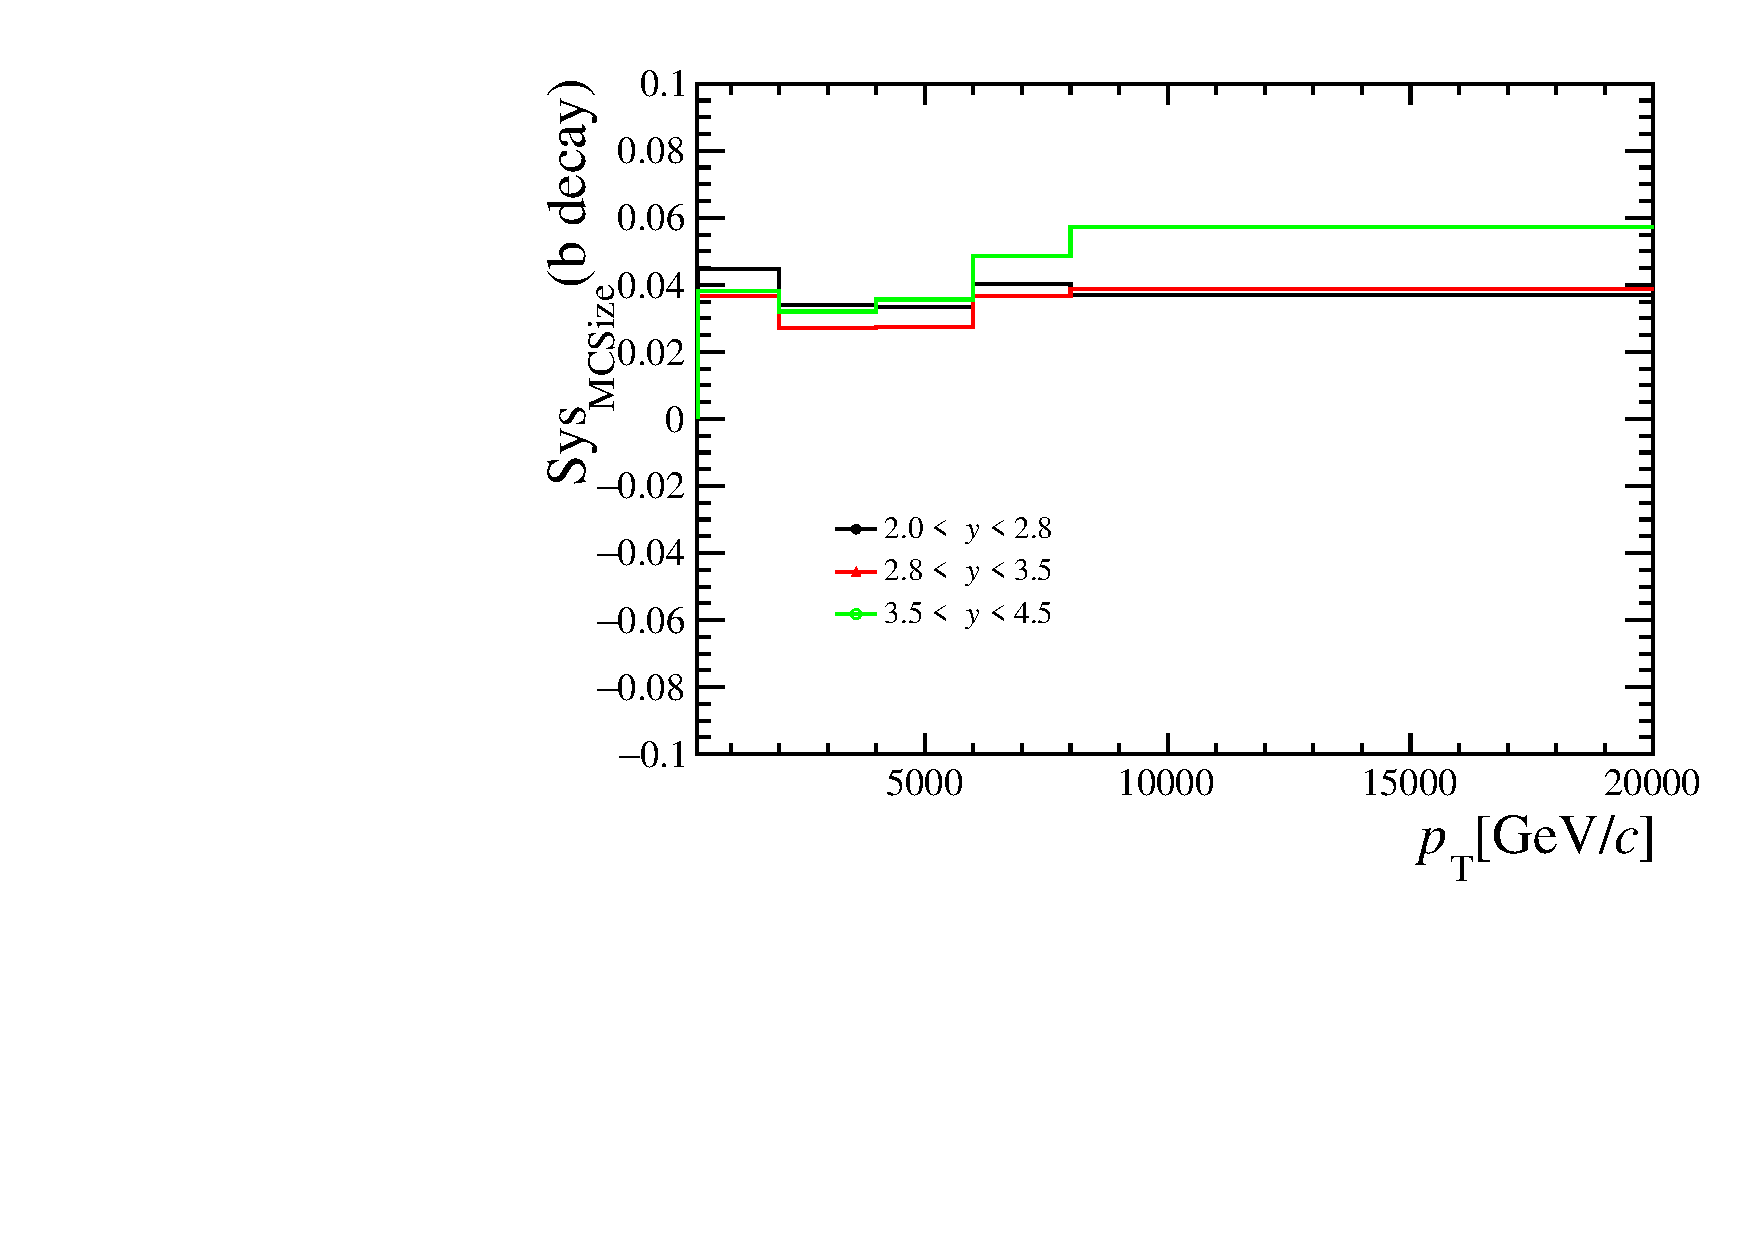
\includegraphics[width=0.49\linewidth]{pdf/SysMCSize/n1Errb_point.pdf}
      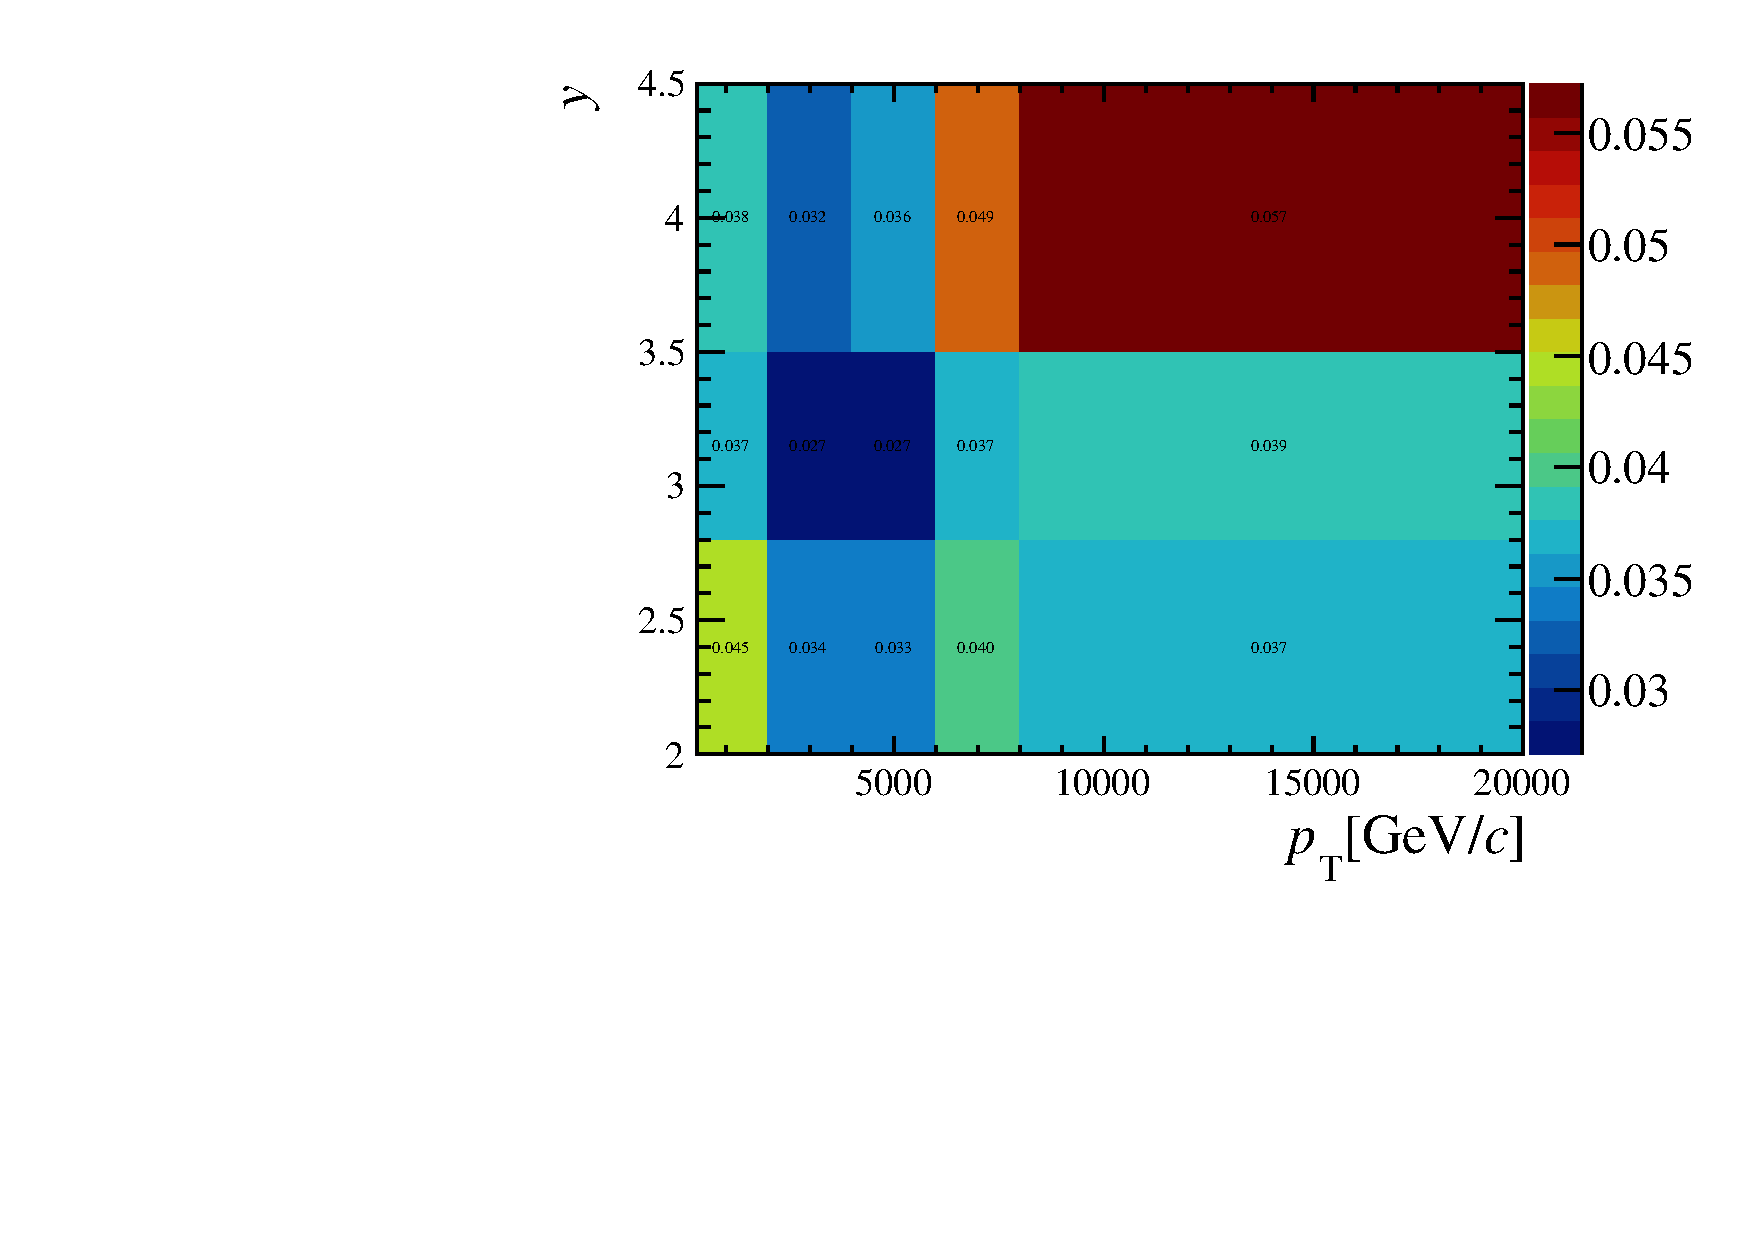
\includegraphics[width=0.49\linewidth]{pdf/SysMCSize/n1Errb.pdf}
    \end{center}
    \caption{The systematic uncertainty of ratio of production due to limit sample size in each bin for PVNTRACKS from 4 to 20. The first row is that of prompt components and the second row is that of components from $b$-hadron decay.
      }
    \label{Sys_MCSize}
\end{figure}

\subsection{Other systematic uncertainties}
\begin{itemize}
\item The uncertainty of $\BR(\jpsi\rightarrow\mu^+\mu^-)=(5.961\pm0.033)\%$ and  $\BR(\psitwos\rightarrow e^+e^-)=(7.93\pm0.17)\times10^{-3}$ are canceled when we only care the normalized ratio.
\item The relative uncertainty of the luminosity is canceled out when calculating the ratio of production cross-section.
\item A fraction of events is lost because of the QED radiative tail. But when calculating the ratio of production, the effects for \jpsi and \psitwos are canceled out.
\end{itemize}
